%%%%%%%%%%%%%%%%%%%%%%%%%%%%%%%%%%%%%%%%%%
% Capstone Project Writeup Draft
% LaTeX Template
% Version 1.0 (November 14, 2024)
% 
% Author:
% Matías Hoyl
%
% License:
% CC BY-NC-SA 4.0 (https://creativecommons.org/licenses/by-nc-sa/4.0/)
%
%%%%%%%%%%%%%%%%%%%%%%%%%%%%%%%%%%%%%%%%%

%----------------------------------------------------------------------------------------
% PACKAGES AND OTHER DOCUMENT CONFIGURATIONS
%----------------------------------------------------------------------------------------

\documentclass[
    a4paper, % Paper size, use either a4paper or letterpaper
    10pt, % Default font size, can also use 11pt or 12pt, although this is not recommended
    % unnumberedsections, % Commented out to enable section numbering
    twoside, % Two side traditional mode where headers and footers change between odd and even pages, comment this option to make them fixed
]{LTJournalArticle}

\usepackage{indentfirst} % Add this line to indent the first paragraph of each section

\usepackage{tabularx}
\usepackage{longtable} % Add longtable package for tables that span multiple pages/columns
\usepackage{dblfloatfix} % Fix issues with double-column floats in two-column documents
\usepackage{float} % Add float package to control float positioning
\usepackage{supertabular} % Add supertabular package for breakable tables across columns
\usepackage{amsmath} % Add amsmath package for \text command and other math features

\addbibresource{references.bib} % BibLaTeX bibliography file

\runninghead{Synthetic Student Responses} % Updated running head

\setcounter{page}{1} % The page number of the first page, set this to a higher number if the article is to be part of an issue or larger work

\usepackage{tcolorbox}
\tcbuselibrary{breakable, skins}

\usepackage{xcolor}

\usepackage{enumitem} % Ensure this package is included

% Explicitly set spacing for enumerate environments
\setlist[enumerate]{noitemsep, topsep=0pt, partopsep=4pt, parsep=4pt}

% Define slate color palette
\definecolor{slate-50}{HTML}{F8FAFC}
\definecolor{slate-100}{HTML}{F1F5F9}
\definecolor{slate-200}{HTML}{E2E8F0}
\definecolor{slate-300}{HTML}{CBD5E1}
\definecolor{slate-400}{HTML}{94A3B8}
\definecolor{slate-500}{HTML}{64748B}
\definecolor{slate-600}{HTML}{475569}
\definecolor{slate-700}{HTML}{334155}
\definecolor{slate-800}{HTML}{1E293B}
\definecolor{slate-900}{HTML}{0F172A}

% Then use the tcolorbox definition as before
\newtcolorbox{promptbox}{
    colback=slate-100,
    colframe=slate-400,
    boxrule=0.5pt,
    arc=2pt,
    fontupper=\ttfamily\footnotesize,
    left=10pt,
    right=10pt,
    top=8pt,
    bottom=8pt,
    breakable
}

% Updated box definitions
\newtcolorbox{questionbox}[2][]{%
    enhanced,
    colback=slate-50,
    colframe=slate-400,
    boxrule=0.5pt,
    arc=4pt,
    title={#2},
    fonttitle=\bfseries\color{white},
    attach boxed title to top left={xshift=0.5cm,yshift=-\tcboxedtitleheight/2},
    boxed title style={
        colback=slate-400,
        colframe=slate-400,
        arc=2pt,
        boxrule=0pt,
    },
    top=12pt, % Increased top padding
    breakable,
    #1
}

\newtcolorbox{studentbox}[2][]{%
    enhanced,
    colback=slate-100,
    colframe=slate-500,
    boxrule=0.5pt,
    arc=4pt,
    title={#2},
    fonttitle=\bfseries\color{white},
    attach boxed title to top left={xshift=0.5cm,yshift=-\tcboxedtitleheight/2},
    boxed title style={
        colback=slate-500,
        colframe=slate-500,
        arc=2pt,
        boxrule=0pt,
    },
    top=12pt,
    breakable,
    #1
}

\newtcolorbox{llmbox}[2][]{%
    enhanced,
    colback=slate-200,
    colframe=slate-600,
    boxrule=0.5pt,
    arc=4pt,
    title={#2},
    fonttitle=\bfseries\color{white},
    attach boxed title to top left={xshift=0.5cm,yshift=-\tcboxedtitleheight/2},
    boxed title style={
        colback=slate-600,
        colframe=slate-600,
        arc=2pt,
        boxrule=0pt,
    },
    top=12pt,
    breakable,
    #1
}

%----------------------------------------------------------------------------------------
% TITLE SECTION
%----------------------------------------------------------------------------------------

% \title{The Artificial Testing Room: Using LLM-Extracted Features to Simulate Student Responses and Predict IRT Difficulty} 

\title{Synthetic Student Responses: LLM-Extracted Features for IRT Difficulty Parameter Estimation}

% Authors are listed in a comma-separated list with superscript numbers indicating affiliations
% \thanks{} is used for any text that should be placed in a footnote on the first page, such as the corresponding author's email, journal acceptance dates, a copyright/license notice, keywords, etc
\author{% 
    Matías Hoyl\textsuperscript{1} 
}

% Affiliations are output in the \date{} command
\date{\footnotesize \textsuperscript{1}School of Education, Stanford University}

\begin{document}

\maketitle

\begin{abstract}
Educational assessment relies heavily on knowing question difficulty, traditionally determined through resource-intensive pre-testing with students. This creates significant barriers for both classroom teachers and assessment developers. We investigate whether Item Response Theory (IRT) difficulty parameters can be accurately estimated without student testing by modeling the response process and explore the relative contribution of different feature types to prediction accuracy. Our approach combines traditional linguistic features with pedagogical insights extracted using Large Language Models (LLMs), including solution step count, cognitive complexity, and potential misconceptions. We implement a two-stage process: first training a neural network to predict how students would respond to questions, then deriving difficulty parameters from these simulated response patterns. Using a dataset of over 250,000 student responses to mathematics questions, our model achieves a Pearson correlation of approximately 0.78 between predicted and actual difficulty parameters on completely unseen questions.
\end{abstract}

%----------------------------------------------------------------------------------------
% SECTION: INTRODUCTION
%----------------------------------------------------------------------------------------
\section{Introduction}

Educational assessment plays a vital role in teaching and learning, but creating high-quality questions requires knowing their difficulty level: how challenging they are for students with different abilities. Currently, determining question difficulty requires extensive pre-testing with students followed by statistical analysis, an approach that is effective but creates significant delays and costs in developing new assessments.

For teachers developing classroom assessments, this process is often impractical, leading to tests with unknown psychometric properties. For large-scale assessment programs, the pre-testing requirement consumes substantial resources and limits the speed at which new content can be developed. Both scenarios highlight the need for methods that can predict question difficulty without requiring actual student testing.

This study addresses two specific research questions:
\begin{itemize}
    \item How effectively can we estimate Item Response Theory difficulty parameters without student testing by modeling the student response process?
    \item To what extent do different feature types (LLM-extracted pedagogical features, linguistic characteristics, and semantic embeddings) contribute to the accuracy of difficulty predictions?
\end{itemize}

Rather than treating difficulty prediction as a direct regression problem, which is what most existing research does, we take an approach that mirrors how difficulty emerges in practice: through patterns of student responses.

Our method combines conventional question features with pedagogical insights extracted using Large Language Models (LLMs). These AI tools analyze questions to identify solution steps, required mathematical skills, cognitive complexity, and potential student misconceptions—aspects typically assessed by human experts. The LLM features function much like an experienced teacher would: reading the question and assessing its difficulty based on intuition and experience, combining multiple pedagogical signals to form a holistic judgment. By embedding this pedagogical knowledge in our predictions, we create a system that better reflects how questions function in educational settings.

The remainder of this paper is organized as follows. Section 2 reviews related work on difficulty prediction, highlighting existing approaches and gaps in the literature. Section 3 describes our dataset, which contains over 250,000 student responses to mathematics questions. Section 4 outlines our methodology, including feature engineering and our neural network architecture. Section 5 presents our experimental results, including the primary model's performance, an RMSE-based efficiency evaluation, and a feature ablation study. Finally, Section 6 discusses the implications of our findings, acknowledges limitations, and suggests directions for future research.

%----------------------------------------------------------------------------------------
% SECTION: RELATED WORK
%----------------------------------------------------------------------------------------
\section{Related Work}

\subsection{Traditional Item Difficulty Estimation}

Traditional approaches to difficulty estimation typically rely on either expert judgment or statistical analysis of student responses. Manual calibration by subject matter experts, while common, has been shown to be inconsistent and subjective \cite{rudner2010implementing, impara1998teachers}. Items developed by experts often perform differently than expected when deployed in real settings.

Statistical calibration through pre-testing with actual students provides more reliable estimates but introduces significant delays before questions can be used operationally. This approach typically applies Item Response Theory (IRT) models to estimate difficulty parameters based on student response patterns \cite{rasch1960}. While effective, this process is time-consuming and resource-intensive, creating a bottleneck in the development of high-quality assessments.

The limitations of these traditional methods have motivated research into automated approaches that can predict item difficulty from the question's textual content, potentially reducing or eliminating the need for extensive pre-testing.

\subsection{Text-based Features for Difficulty Prediction}

Research on text-based difficulty prediction has identified several categories of features that contribute to question complexity.

\subsubsection{Linguistic Features}

Linguistic characteristics of questions are strongly associated with their difficulty. Some studies have extracted lexical, syntactic, and semantic features to predict question complexity \cite{alkhuzaey2023text, choi2020predicting}. Common linguistic features include:

\begin{itemize}
    \item \textbf{Lexical features:} Word count, word frequency, word length, and vocabulary difficulty \cite{yaneva2019predicting, benedetto2020framework}
    \item \textbf{Syntactic features:} Sentence length, syntactic complexity, and grammatical structures \cite{choi2020predicting}
    \item \textbf{Semantic features:} Concept density, abstraction level, and semantic similarity between options \cite{bulut2023evaluating}
\end{itemize}

\textcite{hickendorff2013} demonstrated that linguistic factors significantly impact student performance on mathematics assessments, even when controlling for mathematical complexity.

\subsubsection{Domain-specific Features}

Features specific to certain domains have been shown to improve prediction accuracy:

\begin{itemize}
    \item \textbf{Mathematics:} Number of mathematical symbols, presence of graphs or figures, computation complexity \cite{benedetto2020r2de}
    \item \textbf{Reading comprehension:} Text layout, presence of contextual cues, relationship between passages and questions \cite{lawrence2022reading}
    \item \textbf{Multiple-choice questions:} Similarity between options, plausibility of distractors \cite{kurdi2016experimental, yaneva2018automatic}
\end{itemize}

\textcite{toyama2021makes} emphasized that item difficulty is determined by the interplay of item characteristics, respondent characteristics, and the context in which assessment occurs.

\subsection{Machine Learning Approaches for Difficulty Prediction}

Early approaches to difficulty prediction relied on deterministic methods or simple regression models. Recent advances have introduced increasingly sophisticated machine learning techniques.

\subsubsection{Classical Machine Learning Methods}

Traditional machine learning algorithms have been widely applied to the challenge of difficulty prediction. Linear and logistic regression models have proven effective in establishing relationships between text features and difficulty levels, as demonstrated by \textcite{yaneva2019predicting} in their work on high-stakes medical exams. More sophisticated approaches include the R2DE model proposed by \textcite{benedetto2020r2de}, which leverages random forests to simultaneously predict both IRT difficulty and discrimination parameters based on TF-IDF features extracted from question text. The literature also shows that feature-based ensemble methods have achieved notable success across various educational domains, with \textcite{yaneva2019predicting} demonstrating that combining different feature types can enhance prediction accuracy compared to single-feature approaches.

\subsubsection{Neural Network Models}

Deep learning approaches have increasingly been applied to difficulty prediction, with several notable innovations emerging in recent years. Recurrent Neural Networks, particularly those utilizing Long Short-Term Memory (LSTM) architectures, have demonstrated effectiveness in capturing sequential patterns within question text, as shown in the work of \textcite{huang2017question}. Building on this foundation, \textcite{qiu2019question} introduced a more sophisticated approach with their Document-enhanced Attention Network (DAN), which improves prediction accuracy by enriching questions with relevant domain documents. This contextual enhancement allows the model to better understand the relationship between questions and their subject matter. Further advancing the field, \textcite{xue2020predicting} explored transfer learning techniques, demonstrating that models pre-trained on related tasks such as response time prediction can be effectively fine-tuned for difficulty estimation, leveraging knowledge gained from one educational assessment task to improve performance on another.

\subsubsection{Transformer-based Approaches}

The most recent research has explored transformer-based models for difficulty prediction, leveraging their superior ability to capture contextual relationships. \textcite{benedetto2021transformers} compared BERT and DistilBERT models for difficulty estimation, finding that transformer models outperform previous approaches by up to 6.5\% in terms of RMSE. Building on this work, \textcite{gombert2024predicting} employed scalar-mixed transformer encoders with specialized regression heads, showing significant improvements over baseline models. Further advancing the field, \textcite{kapoor2025prediction} incorporated embeddings from various LLMs (ModernBERT, BERT, and LLAMA) alongside linguistic features, achieving a correlation of 0.77 between true and predicted difficulty.

A key advantage of transformer models is their ability to capture complex semantic relationships within text without requiring extensive feature engineering. \textcite{aradelli2020transformers} demonstrated that fine-tuning pre-trained transformers on domain-specific corpora further enhances prediction accuracy. These approaches represent the current state-of-the-art in difficulty prediction, combining the contextual understanding capabilities of transformer architectures with specialized training techniques to achieve unprecedented levels of accuracy in estimating question difficulty from text alone.

\subsection{Feature Extraction Using Language Models}

Recent studies have explored the use of Large Language Models (LLMs) not just for prediction but also for feature extraction:

\begin{itemize}
    \item \textbf{Procedural complexity:} Using LLMs to quantify the number of steps required to solve problems \textcite{liu2023improving}
    \item \textbf{Skill identification:} Extracting the specific skills required to answer questions \textcite{didolkar2024metacognitive}
    \item \textbf{Cognitive level assessment:} Classifying questions according to Bloom's taxonomy \textcite{scaria2024automated}
    \item \textbf{Misconception analysis:} Identifying potential student misconceptions associated with questions \textcite{sadihin2024proposalml}
\end{itemize}

These approaches leverage the reasoning capabilities of LLMs to extract pedagogically meaningful features that might be difficult to capture through conventional feature engineering approaches.

\subsection{Gaps in Current Research}

Despite significant advances in difficulty prediction methods, two important gaps remain in current research.

First, while transformer-based models have shown remarkable results, often outperforming traditional machine learning approaches by leveraging contextual relationships within question text, there has been limited exploration of using Large Language Models (LLMs) to extract pedagogically meaningful features from questions. Most studies rely on conventional linguistic features or embedding-based approaches, neglecting the potential of LLMs to identify more complex attributes, such as procedural complexity, specific mathematical skills, cognitive levels, and potential misconceptions.

These LLM-extracted features could provide richer signals about question characteristics that are difficult to capture through traditional feature engineering approaches. The few studies that have begun exploring LLM-based feature extraction have shown promising results, but this approach remains underutilized in the difficulty prediction literature.

Second, most current research approaches difficulty prediction as a direct regression problem, where models are trained to predict difficulty parameters directly from question text and features. This direct approach, while intuitive, bypasses a crucial intermediate step: modeling how students with varying ability levels would actually respond to these questions.

Few studies have explored the alternative approach of first simulating student responses to questions and then deriving difficulty parameters from these simulated response patterns. This simulation-based approach offers several advantages over direct prediction. It better mimics the actual process through which question difficulty is determined in real educational settings, allowing difficulty parameters to emerge naturally from student performance patterns rather than being directly predicted. Additionally, it provides a more interpretable model that captures both question characteristics and student abilities, while also producing additional useful metrics beyond difficulty, such as discrimination parameters and expected response patterns.

This gap presents an opportunity to develop more robust difficulty estimation methods. If a model can successfully simulate how students would respond to new questions, it could potentially be applied to any unseen question to estimate difficulty parameters without requiring actual student testing. Such an approach would significantly reduce the resource burden of developing high-quality assessments while maintaining psychometric validity.

The present study addresses both of these gaps by (1) leveraging LLMs to extract complex pedagogical features from questions and (2) developing a neural network model that first predicts student responses and then derives IRT difficulty parameters from these predictions, offering a more comprehensive approach to the difficulty estimation problem.

%----------------------------------------------------------------------------------------
% SECTION: DATA
%----------------------------------------------------------------------------------------
\section{Data}

The dataset for this study comes from Zapien, an adaptive math learning platform in Chile. It includes 251,851 student answers to 4,696 unique math questions, provided by 1,875 students.

Since the original question text and answer options were in Spanish, we first translated them to English using Google's Gemini 2.0 Flash model that excels at translation. This step was crucial for optimizing the performance of the English-based text embedding models used later in our feature engineering.

Next, we established benchmark difficulty values for each question. Using the entire dataset of 251,851 student responses, we applied a standard 1-Parameter Logistic (1PL) Item Response Theory model. This model estimates a difficulty parameter for each question based on the observed patterns of correct and incorrect answers across all students. These benchmark parameters represent the "ground truth" difficulty derived from real student performance.

\begin{figure}[H]
    \centering
    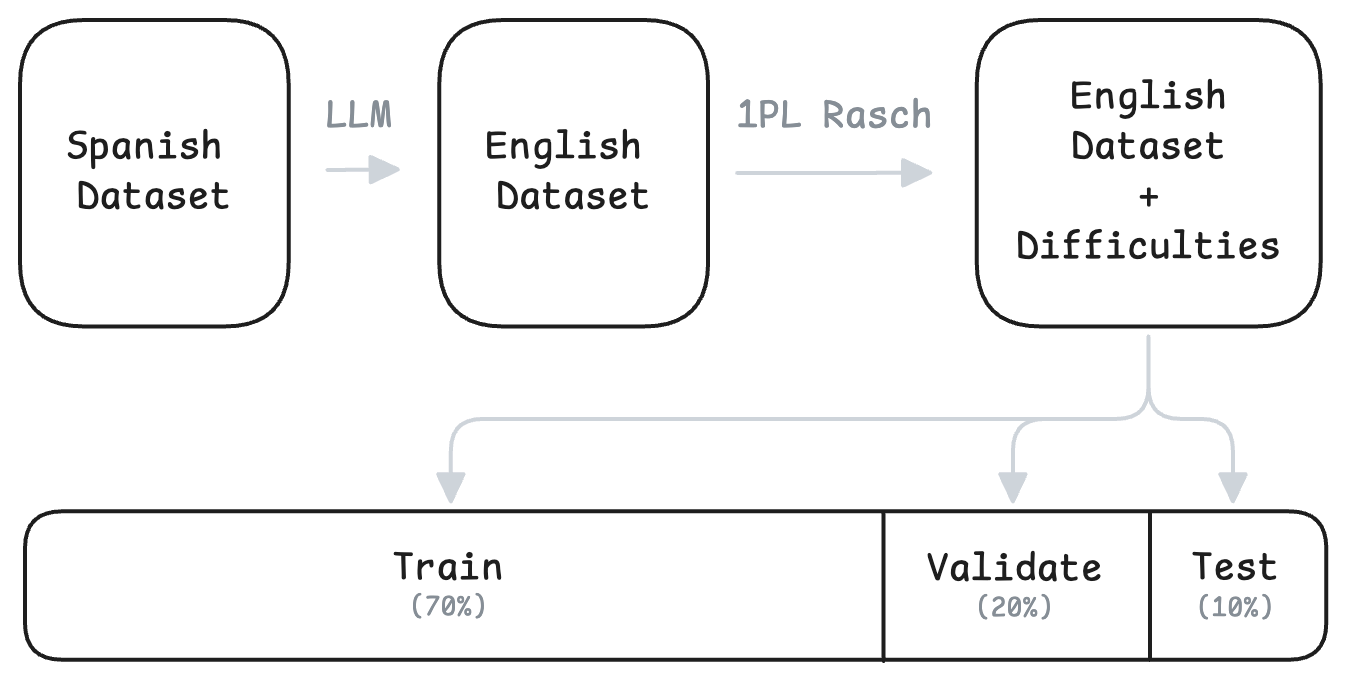
\includegraphics[width=0.8\columnwidth]{figures/data-pipeline.png}
    \caption{Data processing pipeline.}
    \label{fig:data-pipeline}
\end{figure}


Finally, to train and evaluate our prediction model, we split the 4,696 questions into three sets: training (70\%), validation (20\%), and a holdout test set (10\%). This split was done using stratified sampling based on both the difficulty calculated earlier and the average student correctness for each question. Stratification ensures that all three sets have comparable distributions of question difficulty and student performance patterns.

\begin{table}[H] % Keep table floating behavior if desired
    \centering
    \begin{tabular}{lll}
        \hline
        \textbf{Split} & \textbf{Questions} & \textbf{Answers} \\
        \hline
        Training & 3,286 (70\%) & 178,031 (71\%) \\
        Validation & 940 (20\%) & 49,100 (19\%) \\
        Holdout Test & 470 (10\%) & 24,720 (10\%) \\
        \hline
    \end{tabular}
    \caption{Dataset splits.}
    \label{tab:dataset-splits} % Add a label for referencing
\end{table}

% Removed redundant text that is now covered in the narrative above.
% The splits were generated using stratified sampling based on student correctness and original 1PL IRT difficulty to ensure comparable distributions across sets.


%----------------------------------------------------------------------------------------
% SECTION: METHODS
%----------------------------------------------------------------------------------------


\section{Methods}

This section outlines our methodological approach. Our method predicts question difficulty in a two-stage process. First, we train a neural network to predict whether a student will answer a given mathematics question correctly. This network uses three main types of information: (1) student representation (as a vector of features that the model learns from the training data), (2) a rich set of question features (including linguistic characteristics, structural properties, and pedagogical insights extracted by LLMs), and (3) semantic embeddings of the question text itself. Second, we use the network's correctness predictions across many simulated student-question interactions to derive Item Response Theory (IRT) difficulty parameters for each question.

\begin{figure}[H]
    \centering
    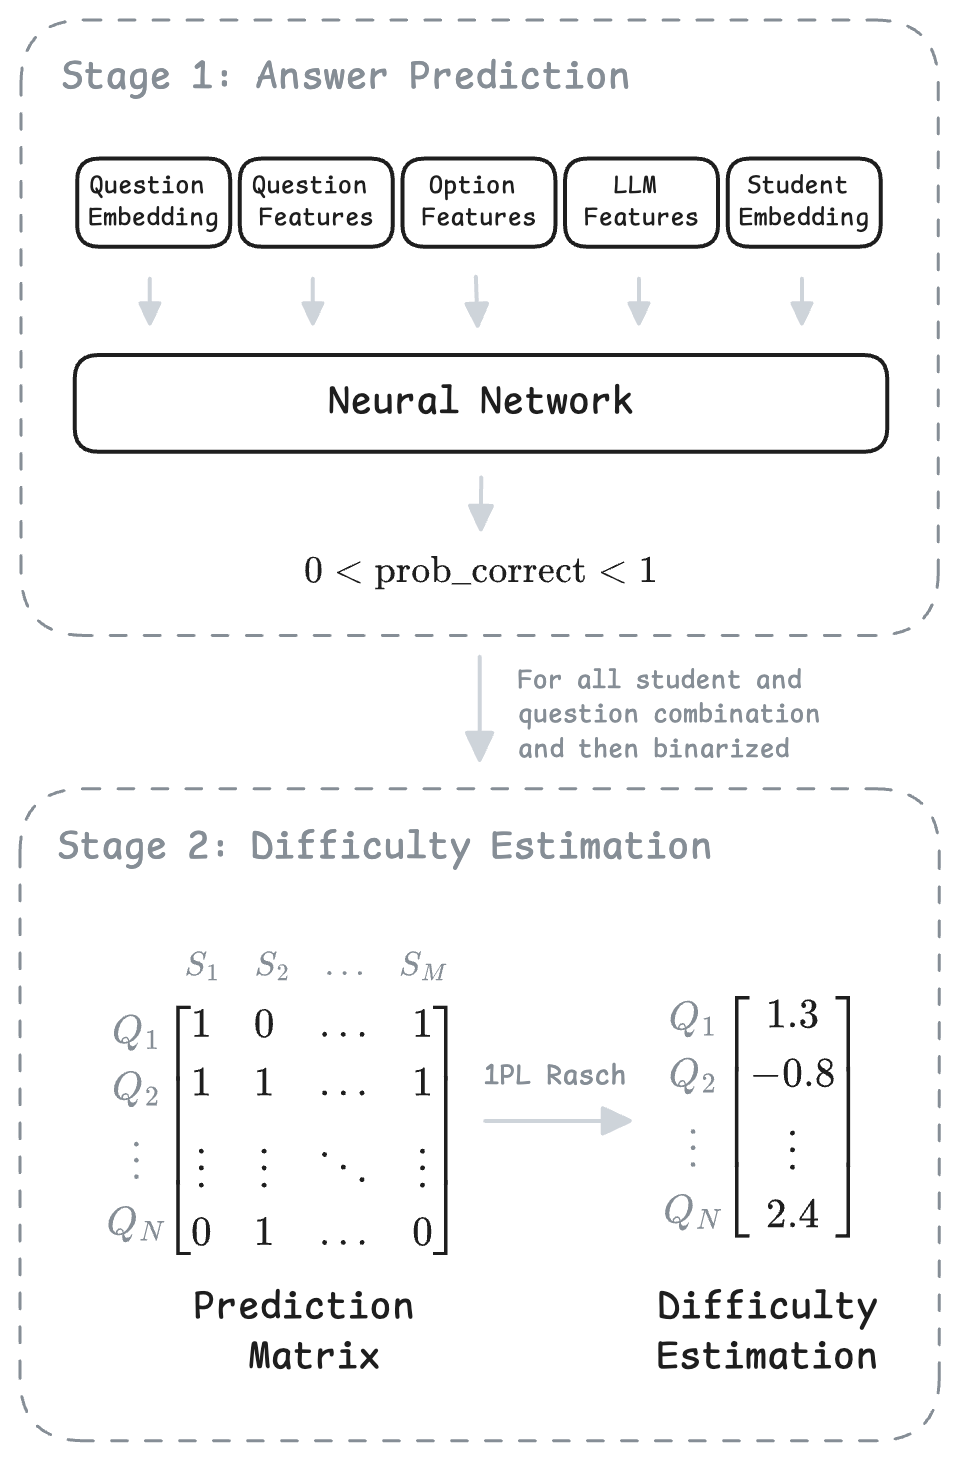
\includegraphics[width=0.8\columnwidth]{figures/full-model.png}
    \caption{Full prediction and estimation pipeline. The neural network makes a prediction for each student-question interaction, then we use the 1PL IRT model to estimate the difficulty parameters using a prediction matrix.}
    \label{fig:model-pipeline}
\end{figure}


\subsection{Stage 1: Neural Network for Correctness Prediction}
Our neural network model is designed to predict the probability of a student answering a question correctly. It takes three primary types of inputs:

\begin{enumerate}
    \item \textbf{Question Embedding}: A 768-dimensional embedding vector representing the formatted question text and answer options.
    \item \textbf{Question Features}: A vector of 48 engineered features capturing question characteristics (linguistic, structural, and LLM-derived pedagogical aspects, including one-hot encoded categorical features).
    \item \textbf{User Embedding}: A learned embedding vector representing the student, for capturing student-question interactions.
\end{enumerate}

\subsubsection{Question Text Embeddings}
To capture the semantic meaning of the entire question context, we generated contextual embeddings for the question title combined with its answer options. The text was formatted as:

    \begin{promptbox}
        \textbf{Question:} [problem\_statement]\\
        \textbf{Correct Answer:} [correct\_option]\\
        \textbf{Wrong Answer 1:} [wrong\_option\_1]\\
        ... \\
        \textbf{Wrong Answer 4:} [wrong\_option\_4]
    \end{promptbox}
    
This formatted text was processed using the \texttt{nomic-ai/modernbert-embed-base} model to generate 768-dimensional embeddings, which were L2 normalized. These serve as a direct input to the neural network.

\subsubsection{Linguistic and Structural Features}
A set of numerical features was engineered to capture textual complexity, mathematical content, and structural characteristics of the questions and their answer options. These features include:
\begin{itemize}
    \item \textbf{From Question Title/Text:} \texttt{question\_word\_count}, \texttt{question\_char\_count}, \texttt{question\_avg\_word\_length}, \texttt{question\_digit\_count}, \texttt{question\_special\_char\_count}, \texttt{question\_mathematical\_symbols}, \texttt{question\_latex\_expressions}.
    \item \textbf{From Answer Options:} \texttt{jaccard\_similarity\_std} (standard deviation of Jaccard similarities between option pairs), \texttt{avg\_option\_length}, \texttt{avg\_option\_word\_count}, \texttt{Answer\_Length\_Variance}, \texttt{Has\_NoneAll\_Option} (binary, treated as numerical), \texttt{Option\_Length\_Outlier\_Flag} (binary, treated as numerical).
    \item \textbf{Structural/Metadata:} \texttt{has\_image} (binary, treated as numerical).
\end{itemize}
These features are part of the \texttt{BASE\_NUMERICAL\_FEATURE\_COLS} used in our primary model script.



\subsubsection{Options Embeddings and Derived Features}
While individual option embeddings were also generated using \texttt{nomic-ai/modernbert-embed-base} for each answer choice (A through E), these raw embeddings were not directly fed into separate pathways in the final neural network. Instead, specific numerical features were pre-calculated from these option embeddings and included in the \texttt{BASE\_NUMERICAL\_FEATURE\_COLS}. These derived features are:
\begin{itemize}
    \item \textbf{Correct\_Distractor\_CosineSim\_Mean:} The mean cosine similarity between the embedding of the correct option and the embeddings of each incorrect (distractor) option.
    \item \textbf{Distractor\_Embedding\_Distance\_Mean:} The mean Euclidean distance between the embeddings of all pairs of distractor options.
\end{itemize}
These metrics provide insights into the semantic similarity between the correct answer and distractors, and among the distractors themselves.

\subsubsection{Feature Extraction Using LLMs}
We utilized Google's Gemini models (primarily \texttt{gemini-2.0-flash} for simpler feature extractions and \texttt{gemini-2.5-flash} or \texttt{gemini-2.5-pro} for more complex ones like archetype classification, as detailed in Appendix \ref{app:llm_prompts}) to extract pedagogically relevant features from the question text and, where applicable, provided solutions. To ensure stability and mitigate the probabilistic nature of LLMs, features were typically generated over N runs (e.g., 3 runs for numerical estimates like information gap, or 1 run for simpler classifications) and then aggregated (e.g., by averaging numerical values or using the mode for categorical ones). The prompts used aimed to elicit chain-of-thought reasoning from the LLM before providing the final structured JSON output. It is important to note that while a broader range of pedagogical features (such as a detailed taxonomy of mathematical skills) were explored during development, the final reported model incorporates the LLM-derived features listed below.

\paragraph{Procedural Complexity and Cognitive Demand}
\begin{itemize}
    \item \textbf{avg\_steps}: The average number of discrete, pedagogically atomic solution steps required to solve the question, determined by LLM analysis of the solution process (averaged over 3 runs). The prompt guided the LLM to break down solutions in a manner appropriate for student instruction (see Appendix \ref{app:prompt_avg_steps} for a conceptual prompt example, specific prompt for this automated feature might differ but follows this intent).
    \item \textbf{level}: The primary cognitive level assessed by the question, based on Bloom's Taxonomy (1-6, see Appendix \ref{tab:blooms-taxonomy}), determined by LLM analysis (majority vote over 3 runs). This is an ordinal feature treated as numerical. (See Appendix \ref{app:prompt_bloom} for the conceptual prompt framework).
    \item \textbf{num\_misconceptions}: The average number of potential student misconceptions associated with the question, identified by the LLM (averaged over 3 runs). The prompt asked for an exhaustive, atomic list (see Appendix \ref{app:prompt_misconceptions} for a conceptual prompt framework).
\end{itemize}

\paragraph{Mathematical and Symbolic Content Features (LLM-derived)}
\begin{itemize}
    \item \textbf{Mathematical\_Notation\_Density}: An LLM-derived measure assessing the density or complexity of mathematical notation. (While related to nesting depth, specific extraction might involve a nuanced prompt focusing on overall symbolic density, see Appendix \ref{app:prompt_nesting_depth} for the related nesting depth prompt which captures aspects of this).
    \item \textbf{Max\_Expression\_Nesting\_Depth}: The maximum nesting depth of mathematical expressions (e.g., parentheses, functions, fractions) found in the question, determined by LLM analysis (mode over 3 runs, see Appendix \ref{app:prompt_nesting_depth}).
    \item \textbf{Ratio\_Abstract\_Concrete\_Symbols}: The ratio of abstract symbols (variables) to concrete numerical values in the question, calculated from LLM counts (see Appendix \ref{app:prompt_abstract_ratio}).
    \item \textbf{Has\_Abstract\_Symbols}: Binary indicator (1/0) if abstract symbols (beyond common variables) are present, determined by LLM analysis (1 run, see Appendix \ref{app:prompt_has_abstract_symbols}).
    \item \textbf{Units\_Check}: Binary indicator (1/0) if checking or converting units is significantly involved, determined by LLM analysis (1 run, see Appendix \ref{app:prompt_units_check}).
\end{itemize}

\paragraph{Question-Answer Relationship and Context Features (LLM-derived)}
\begin{itemize}
    \item \textbf{Question\_Answer\_Info\_Gap}: An LLM-estimated measure (1-4 scale) of the information gap between the question stem and the knowledge needed to derive the answer (averaged over 3 runs, see Appendix \ref{app:prompt_info_gap}).
    \item \textbf{RealWorld\_Context\_Flag}: Binary indicator (1/0) if the question is set in a real-world context versus purely abstract, determined by LLM analysis (1 run, see Appendix \ref{app:prompt_realworld_flag}).
\end{itemize}

\paragraph{Distractor Plausibility Features (LLM-derived)}
\begin{itemize}
    \item \textbf{LLM\_Distractor\_Plausibility\_Max}: The average (over 3 runs) of the maximum plausibility scores (1-5 scale) assigned by an LLM among the distractor options for a given question (see Appendix \ref{app:prompt_distractor_plausibility}).
    \item \textbf{LLM\_Distractor\_Plausibility\_Mean}: The average (over 3 runs) of the mean plausibility scores (1-5 scale) assigned by an LLM to the distractor options for a given question (see Appendix \ref{app:prompt_distractor_plausibility}).
    \item \textbf{Extreme\_Wording\_Option\_Count}: Count of options containing extreme wording (e.g., "always", "never"). (This feature might be rule-based or LLM-derived; if LLM-derived, a specific prompt would assess this, otherwise it's pattern matching.)
\end{itemize}

\paragraph{Categorical Pedagogical Features (LLM-derived, One-Hot Encoded)}
The following LLM-derived features were treated as categorical and subsequently one-hot encoded before being fed into the neural network:
\begin{itemize}
    \item \textbf{Knowledge\_Dimension}: The primary dimension of knowledge assessed (Factual, Conceptual, or Procedural), determined by LLM analysis (1 run, see Appendix \ref{app:prompt_knowledge_dimension}).
    \item \textbf{Most\_Complex\_Number\_Type}: The highest level of numerical complexity (1-5 scale: Integer to Complex Number) present in the question or options, determined by LLM analysis (1 run, see Appendix \ref{app:prompt_complex_number_type}).
    \item \textbf{Problem\_Archetype}: The general type or structure of the problem (e.g., Word Problem - Calculation, Equation Solving), determined by LLM analysis using \texttt{gemini-2.5-pro} (1 run, see Appendix \ref{app:prompt_problem_archetype}).
\end{itemize}
The combination of the raw numerical features listed above (linguistic, structural, LLM-derived numerical/binary) and the one-hot encoded versions of these three categorical features results in the 48 final numerical input features for the neural network.

\subsubsection{User Embeddings}

The last piece of the puzzle in our modeling approach was incorporating user information, since we had student answer data for each question. Accounting for individual student abilities was essential for accurate predictions, but presented significant technical challenges. We initially attempted to incorporate user IDs as one-hot encoded features in a LightGBM model, but this approach proved problematic. With 1,867 binary features for users compared to only 146 question-related features, the model essentially functioned as a user classifier rather than a question difficulty estimator. This structural imbalance resulted in predictions with minimal variation across questions for the same user (standard deviation only 0.026), compromising our ability to assess question characteristics.

To address this limitation, we implemented a neural network with a dedicated user embedding layer that mapped each user ID to an 8-dimensional vector space. This approach reduced the feature dimensionality while creating dense, continuous representations of user abilities. The embedding layer contained a learnable matrix of dimensions $(n\_users \times embedding\_dim)$ that captured latent ability factors conventional one-hot encoding could not efficiently represent. This embedding-based approach successfully balanced user and question influences, enabling our model to make meaningfully different predictions for different questions presented to the same user, while ensuring user characteristics did not overshadow the question features we were primarily interested in analyzing.

\subsection{Modeling Approach}

Our neural network model is designed to predict the probability of a student answering a question correctly. It takes three primary types of inputs:
\begin{enumerate}
    \item \textbf{User Input}: An embedding vector representing the student.
    \item \textbf{Numerical Input}: A vector of 48 engineered features capturing question characteristics (linguistic, structural, and LLM-derived pedagogical aspects, including OHE categorical features).
    \item \textbf{Text Embedding Input}: A 768-dimensional embedding vector representing the formatted question text.
\end{enumerate}

The architecture (as detailed in \texttt{modules/neural\_net.py} and configured by \texttt{run\_best\_model\_no\_filter.py}) is as follows:
\begin{itemize}
    \item The user ID is passed through an embedding layer (8-dimensional output), followed by flattening and a dropout layer (rate 0.25).
    \item The 48 numerical features are processed by a dense layer (32 units, ReLU activation, L2 regularization of 0.0005), followed by a dropout layer (rate 0.25).
    \item The 768-dimensional question text embedding is processed by a dense layer (32 units, ReLU activation, L2 regularization of 0.0005), followed by a dropout layer (rate 0.25).
    \item The outputs of these three pathways are concatenated.
    \item This concatenated vector is then passed through two shared dense layers (64 units and then 32 units, both with ReLU activation, L2 regularization of 0.0005, and dropout rate of 0.25 after each).
    \item The final layer is a single dense unit with a sigmoid activation function to output the probability of a correct answer.
\end{itemize}

\begin{table}[H]
    \centering
    \begin{tabular}{ll}
        \hline
        \textbf{Component/Hyperparameter} & \textbf{Value/Setting} \\
        \hline
        User Embedding Dimension & 8 \\
        Dense Layer Units (Input Pathways) & 32 (for numerical features), 32 (for text embeddings) \\
        Dense Layer Units (Shared) & 64, then 32 \\
        Activation Function (Hidden Layers) & ReLU \\
        L2 Regularization (All weight matrices) & 0.0005 \\
        Dropout Rate (All dropout layers) & 0.25 \\
        Optimization & Adam optimizer \\
        Learning Rate & 0.0002 (2e-4) \\
        Loss Function & Binary cross-entropy  \\
        Metrics & Accuracy, AUC \\
        Batch Size & 1024 \\
        Maximum Epochs & 60 \\
        Early Stopping Patience & 12 (monitors \texttt{val\_loss}) \\
        Restore Best Weights (Early Stopping) & True \\
        \hline
    \end{tabular}
    \caption{Neural network architecture and training hyperparameters for the best performing model (\texttt{config\_F\_lower\_lr\_more\_patience}).}
    \label{tab:model-details}
\end{table}

\subsection{Prediction Task}

After training the neural network on 70\% of the questions and validating on 20\%, we used the model to generate predictions for the 10\% completely unseen questions in the holdout test set. For each of the 470 holdout questions, we generated predictions for all unique users present in the training/validation data (approximately 1,862 users were involved in the final prediction matrix for the test questions as per the ablation script logs). We first preserved the raw probability outputs from the model, representing each student's likelihood of answering correctly. We then applied a 0.5 threshold to these probabilities to convert them to binary predictions (0 for incorrect, 1 for correct). This conversion produced a correctness matrix where each cell contained either 0 or 1.

We then used these binarized correctness matrices as inputs to an Item Response Theory estimation process. We implemented a 1-Parameter Logistic (1PL) IRT model to estimate question difficulty parameters. The parameter estimation employed a maximum likelihood approach using TensorFlow.


%----------------------------------------------------------------------------------------
% SECTION: RESULTS
%----------------------------------------------------------------------------------------
\section{Results}

\subsection{Model Performance}

Our neural network model achieved strong performance in predicting student correctness. The following metrics were obtained on the holdout test set (470 questions) using the best performing model configuration (\texttt{config\_F\_lower\_lr\_more\_patience}):

\begin{table}[H]
    \centering
    \begin{tabular}{lc}
        \hline
        \textbf{Metric} & \textbf{Value} \\
        \hline
        Accuracy & 0.7529 \\
        AUC-ROC & 0.7789 \\
        Precision & 0.8010 \\
        Recall & 0.8719 \\
        F1 Score & 0.8350 \\
        \hline
    \end{tabular}
    \caption{Classification performance metrics on the holdout test set.}
    \label{tab:classification-metrics-test}
\end{table}

These metrics indicate the model's robust ability to predict student responses on unseen questions, providing a solid foundation for the subsequent IRT parameter estimation from these predictions.

\subsection{IRT Parameter Estimation}

Our primary objective was to estimate 1-Parameter Logistic (1PL) IRT difficulty parameters from the neural network's binarized predictions on the holdout test set. The alignment between these NN-derived difficulty parameters and the benchmark 1PL IRT difficulty parameters (calculated from the full original student response dataset) is shown below for our best performing full-feature model (equivalent to Model 4 in the ablation study):

\begin{table}[H]
    \centering
    \begin{tabular}{lc}
        \hline
        \textbf{Metric} & \textbf{Value} \\
        \hline
        Pearson correlation & 0.7791 \\
        Spearman rank correlation & 0.7606 \\
        Number of common questions & 470 \\
        % MAE & [To be added if available for 1PL] \\
        % RMSE (direct, unaligned) & [To be added if available for 1PL] \\
        \hline
    \end{tabular}
    \caption{1PL IRT difficulty parameter estimation metrics on the holdout test set for the full feature model.}
    \label{tab:irt-metrics-1pl}
\end{table}

The high correlation values demonstrate a strong positive relationship between the difficulty parameters estimated via our modeling approach and those derived from actual student response data.

\begin{figure}[H]
    \centering
    % USER: Please ensure 'difficulty_scatter_Model_4_Full.png' (or similar name from your script's output)
    % is placed in a 'figures' subdirectory relative to main.tex, or update path.
    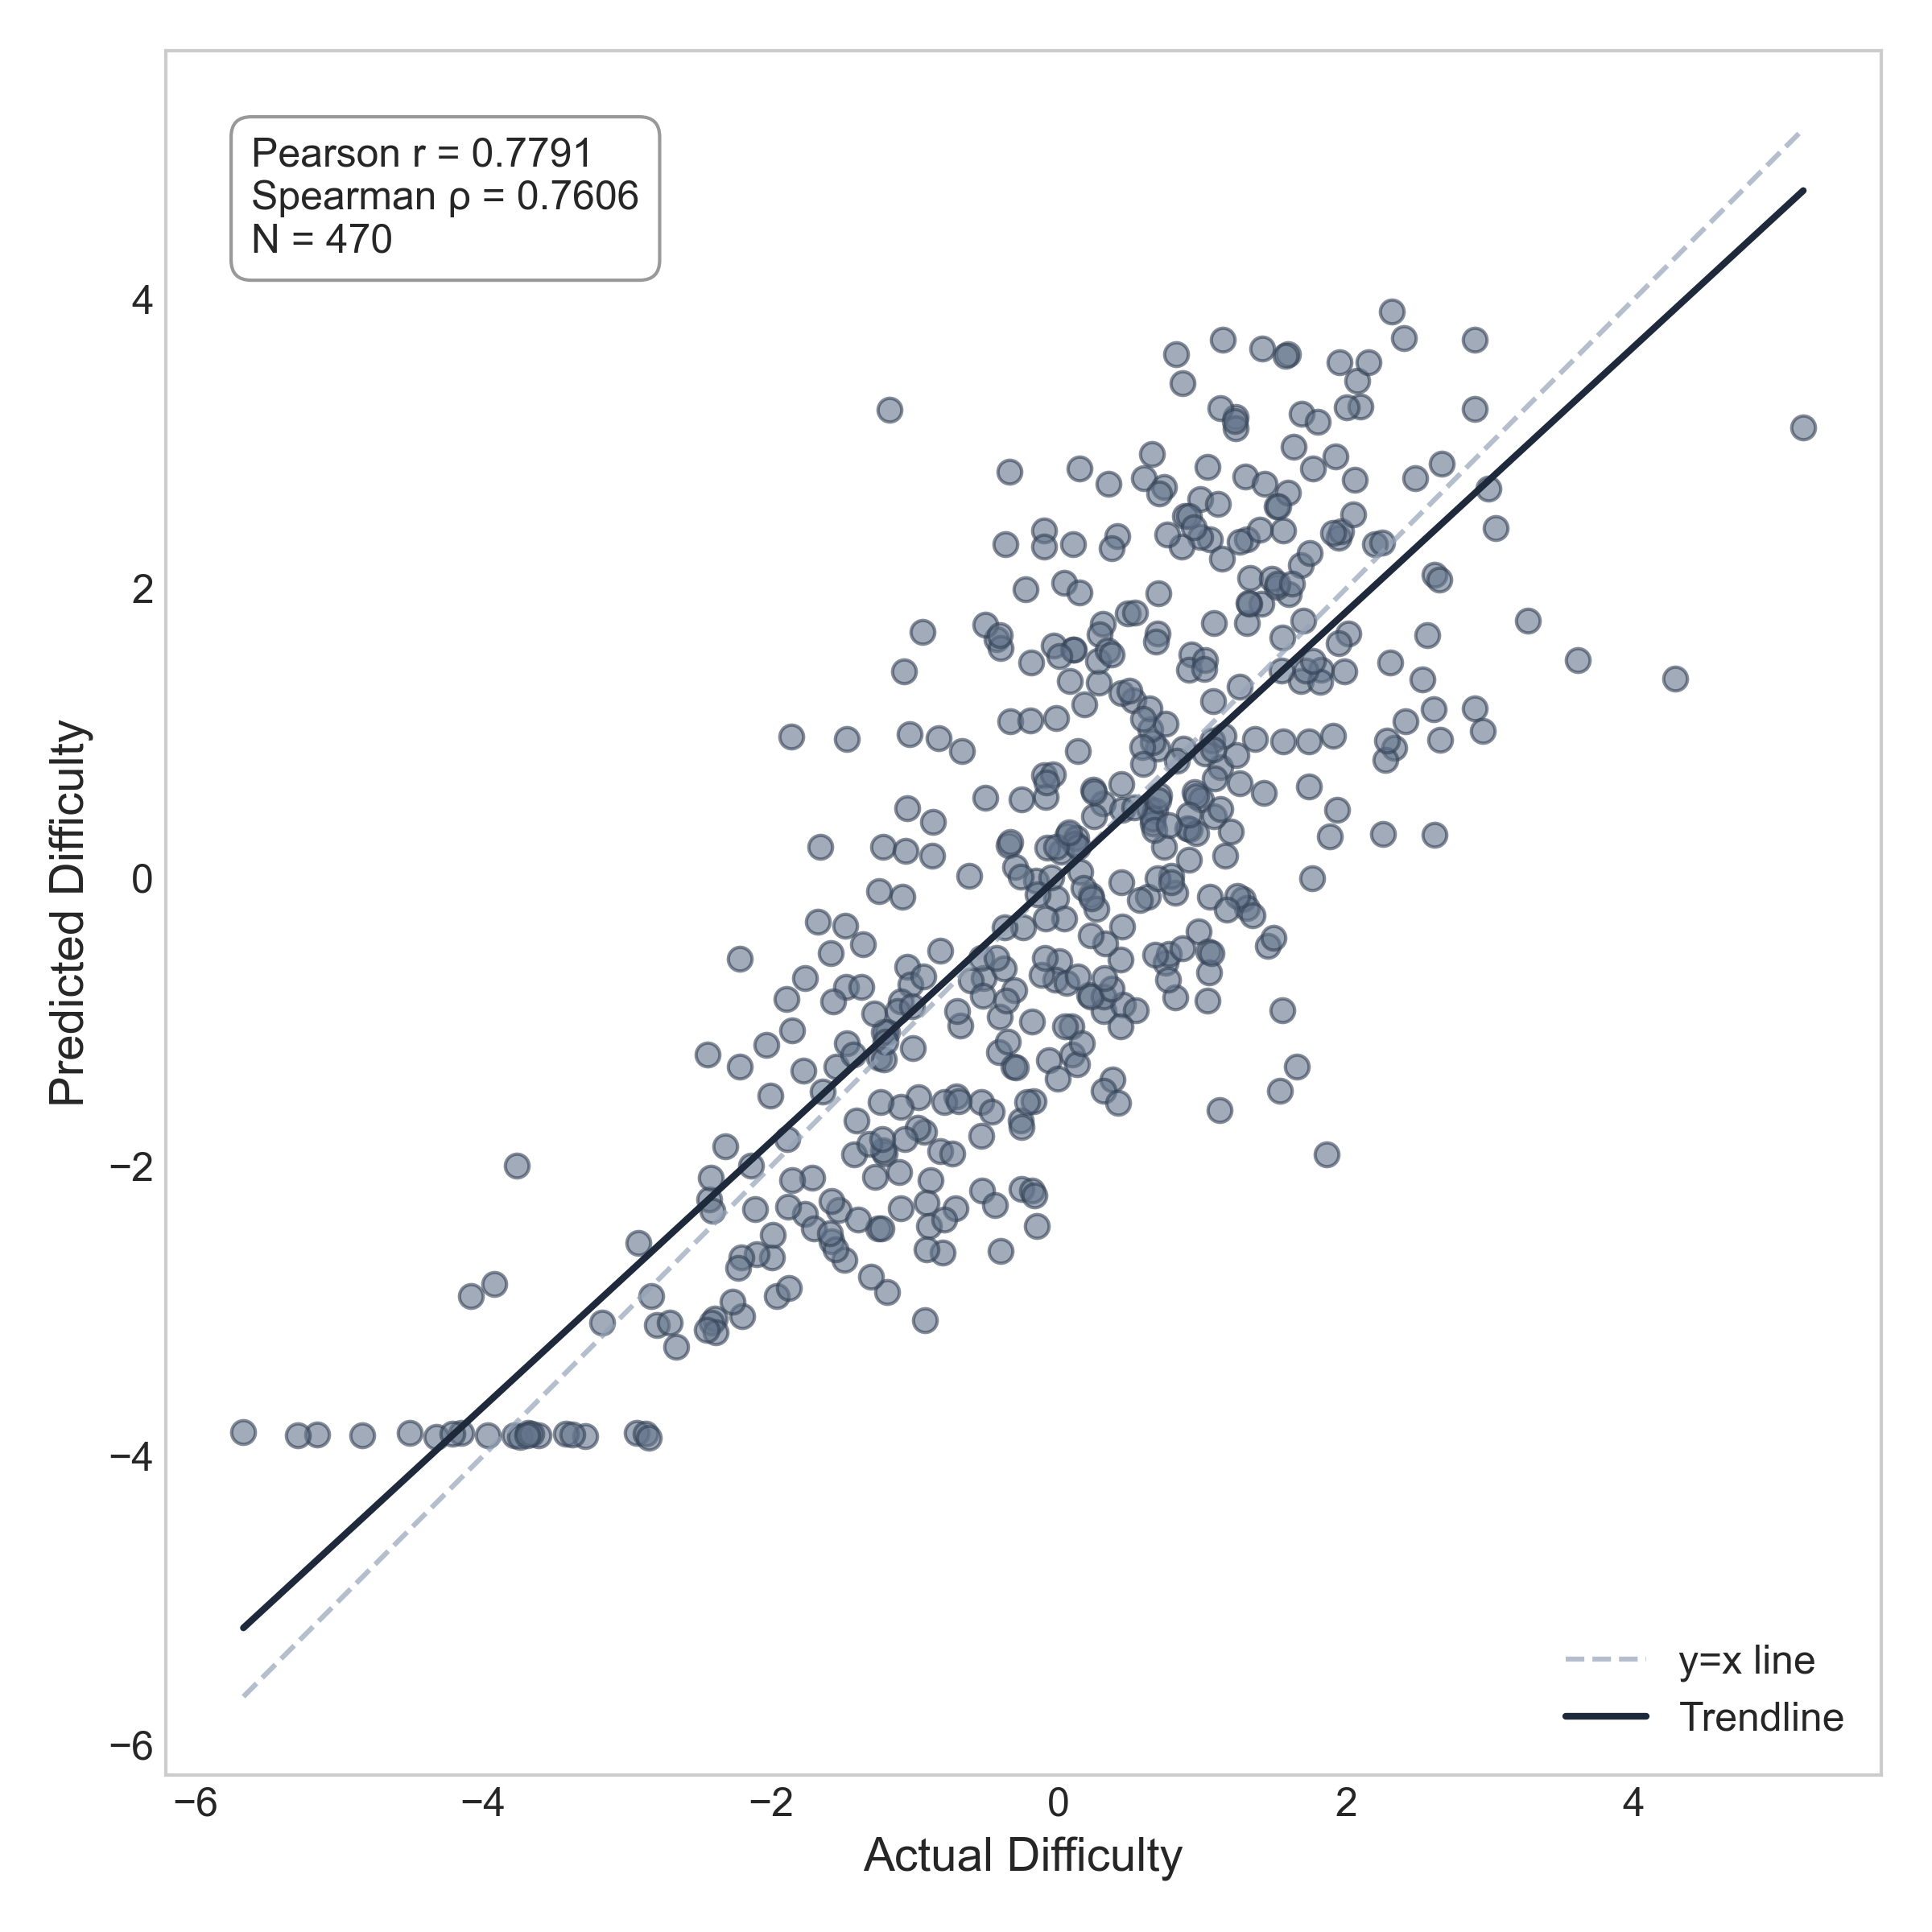
\includegraphics[width=0.8\columnwidth]{figures/difficulty_scatter_Model_4_Full.png} 
    \caption{Correlation between benchmark 1PL IRT difficulty and NN-derived 1PL difficulty (Model 4 - Full Features) on the holdout test set.}
    \label{fig:difficulty-correlation-1pl}
\end{figure}

As shown in Figures \ref{fig:difficulty-correlation-1pl} and \ref{fig:difficulty-distribution-1pl}, our model captures both the relative ordering and, to a good extent, the distribution of question difficulties.

\begin{figure}[H]
    \centering
    % USER: Please ensure 'difficulty_density_Model_4_Full.png' (or similar name from your script's output)
    % is placed in a 'figures' subdirectory relative to main.tex, or update path.
    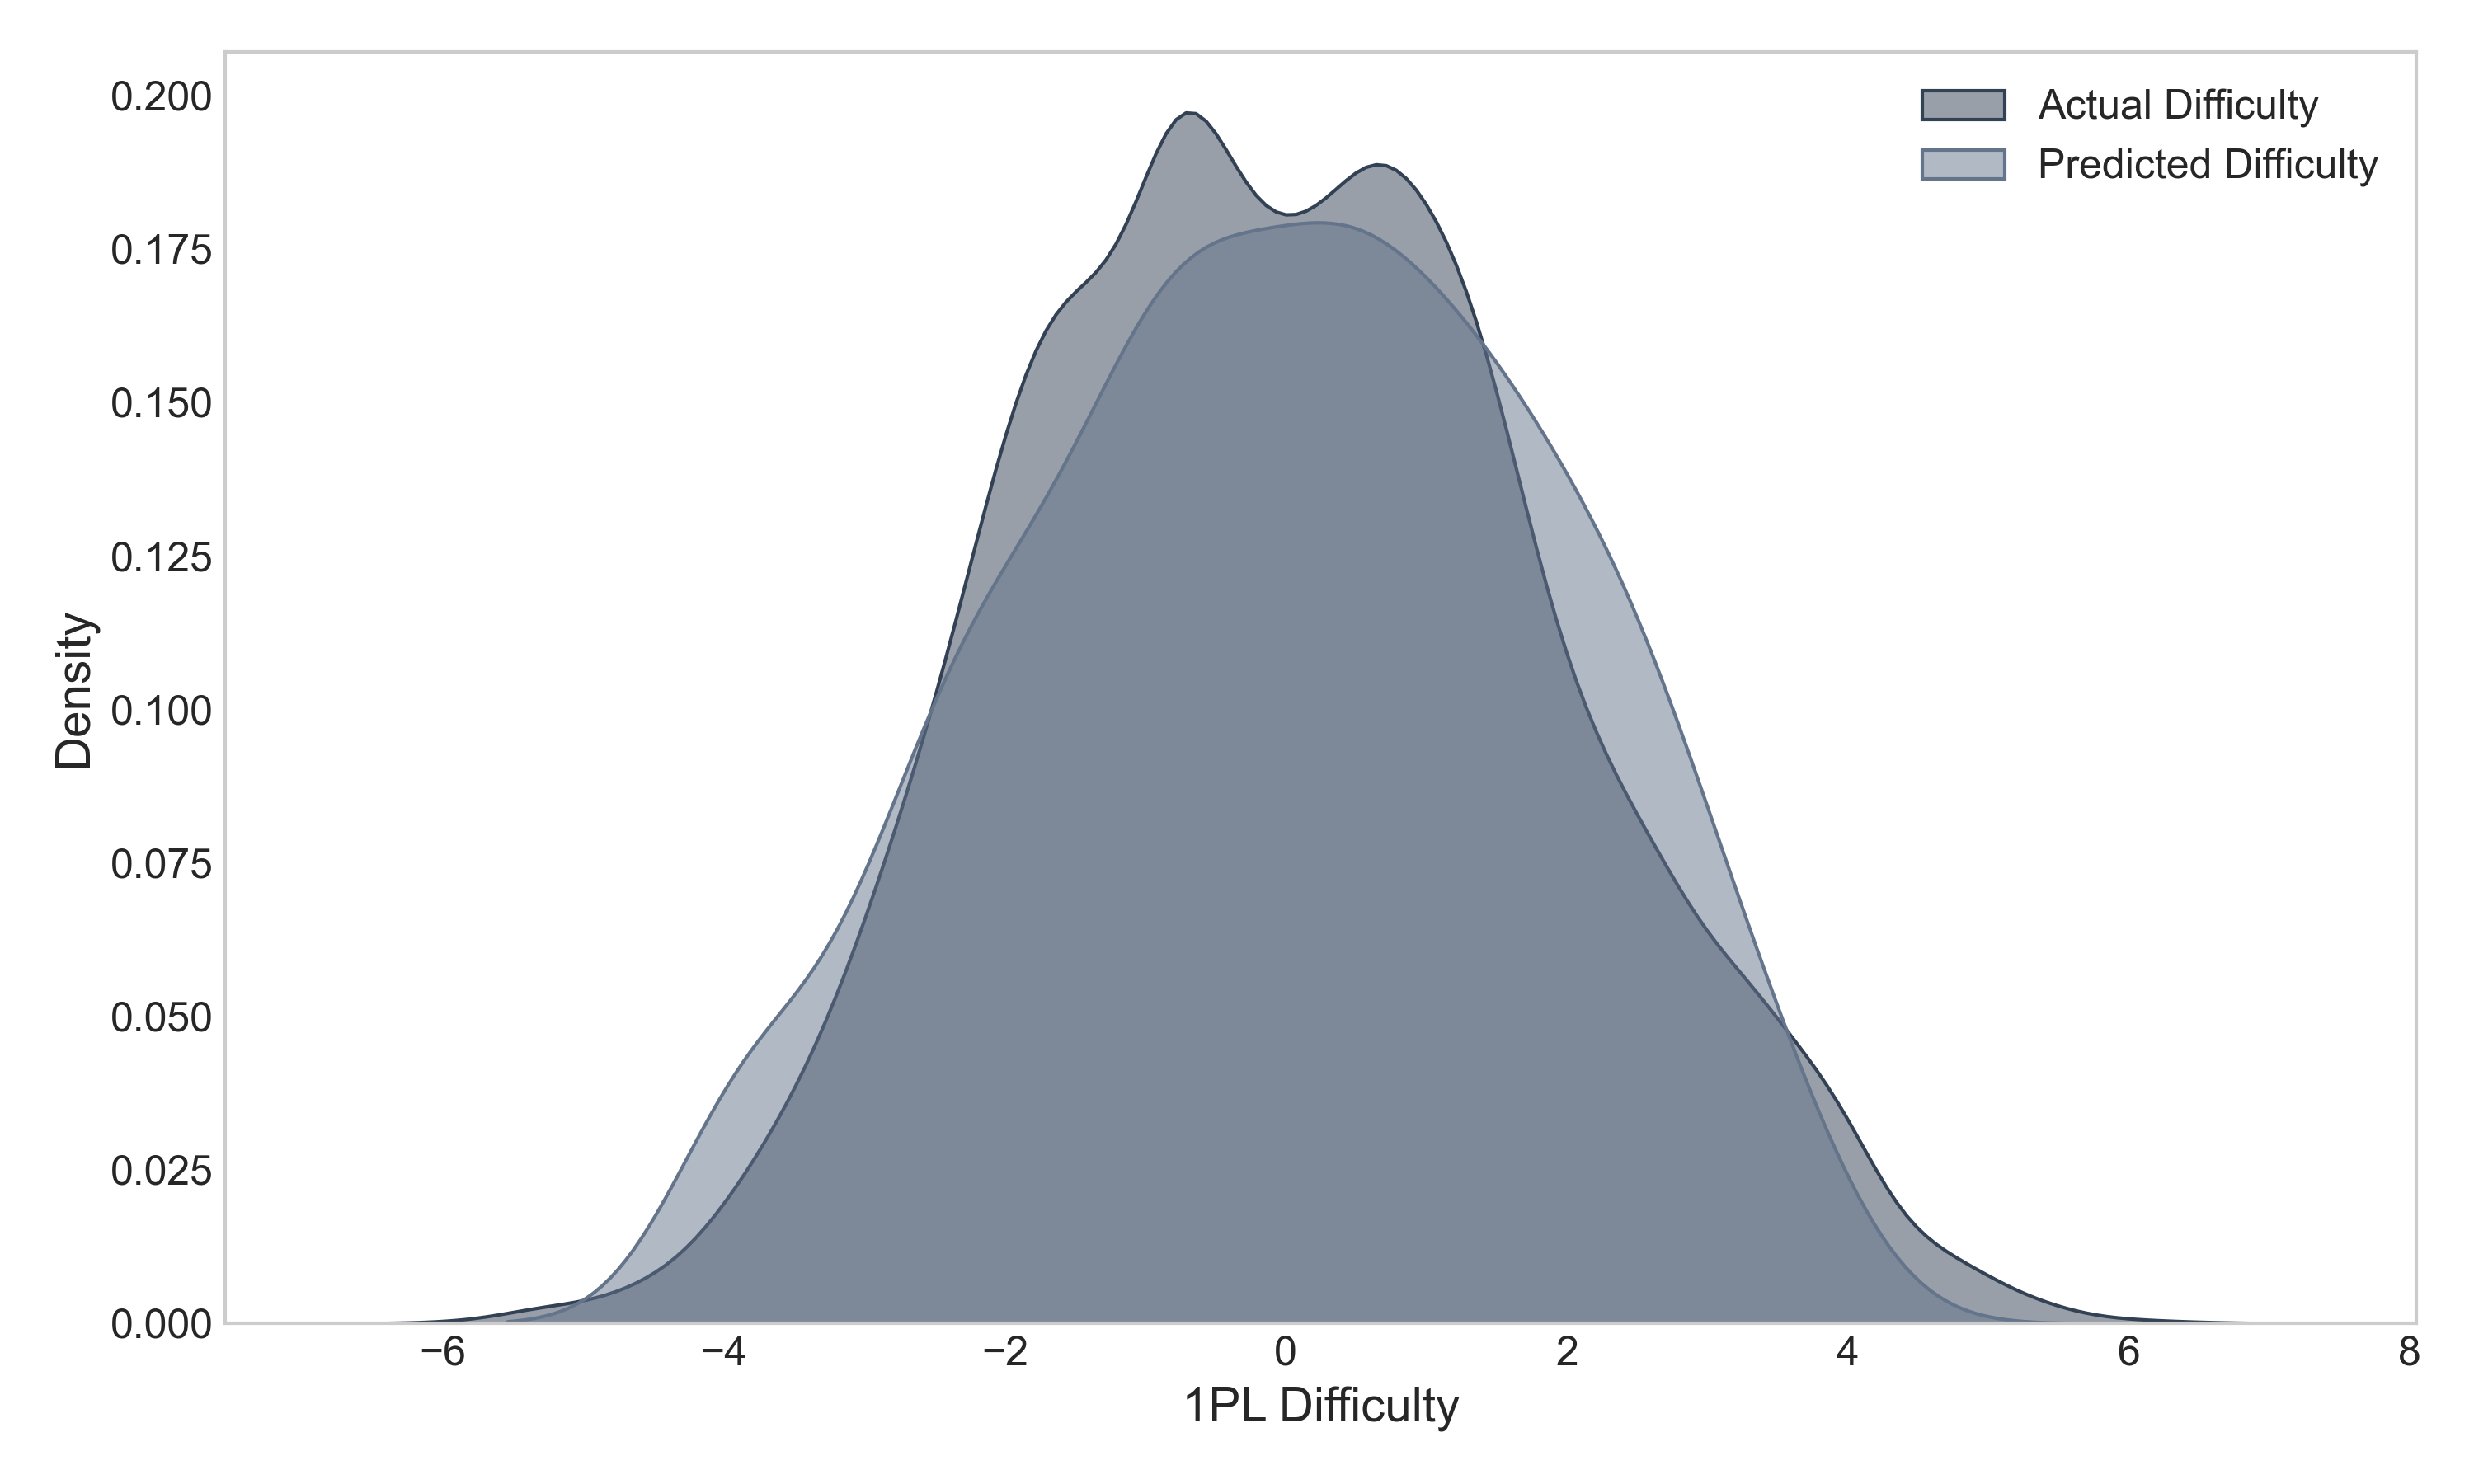
\includegraphics[width=1\columnwidth]{figures/difficulty_density_Model_4_Full.png} 
    \caption{Distribution comparison of benchmark 1PL IRT difficulty and NN-derived 1PL difficulty (Model 4 - Full Features) for the holdout test set.}
    \label{fig:difficulty-distribution-1pl}
\end{figure}

\subsection{RMSE-Based Efficiency Evaluation}
To further contextualize the performance of our NN-derived 1PL difficulty parameters, we conducted an RMSE-based efficiency evaluation. This analysis compares the accuracy of our model's difficulty estimates to those obtainable from traditional 1PL IRT estimations using varying amounts of real student data for the same 470 holdout questions. The ground truth for this comparison was established by calculating 1PL IRT difficulty parameters using all available answers for these 470 questions from the original unfiltered dataset.

After aligning the scale (mean and standard deviation) of our NN-derived 1PL difficulties to these ground truth difficulties, the \textbf{NN-Derived 1PL Model RMSE was 1.1857}.

Figure \ref{fig:rmse-efficiency} illustrates this comparison, showing the RMSE achieved by traditional 1PL IRT with different sample sizes against our model's performance. Table \ref{tab:rmse-efficiency} provides a subset of these data points.

\begin{figure}[H]
    \centering
    % USER: Please ensure 'rmse_efficiency_curve.png' is placed in a 'figures' subdirectory relative to main.tex, or update path.
    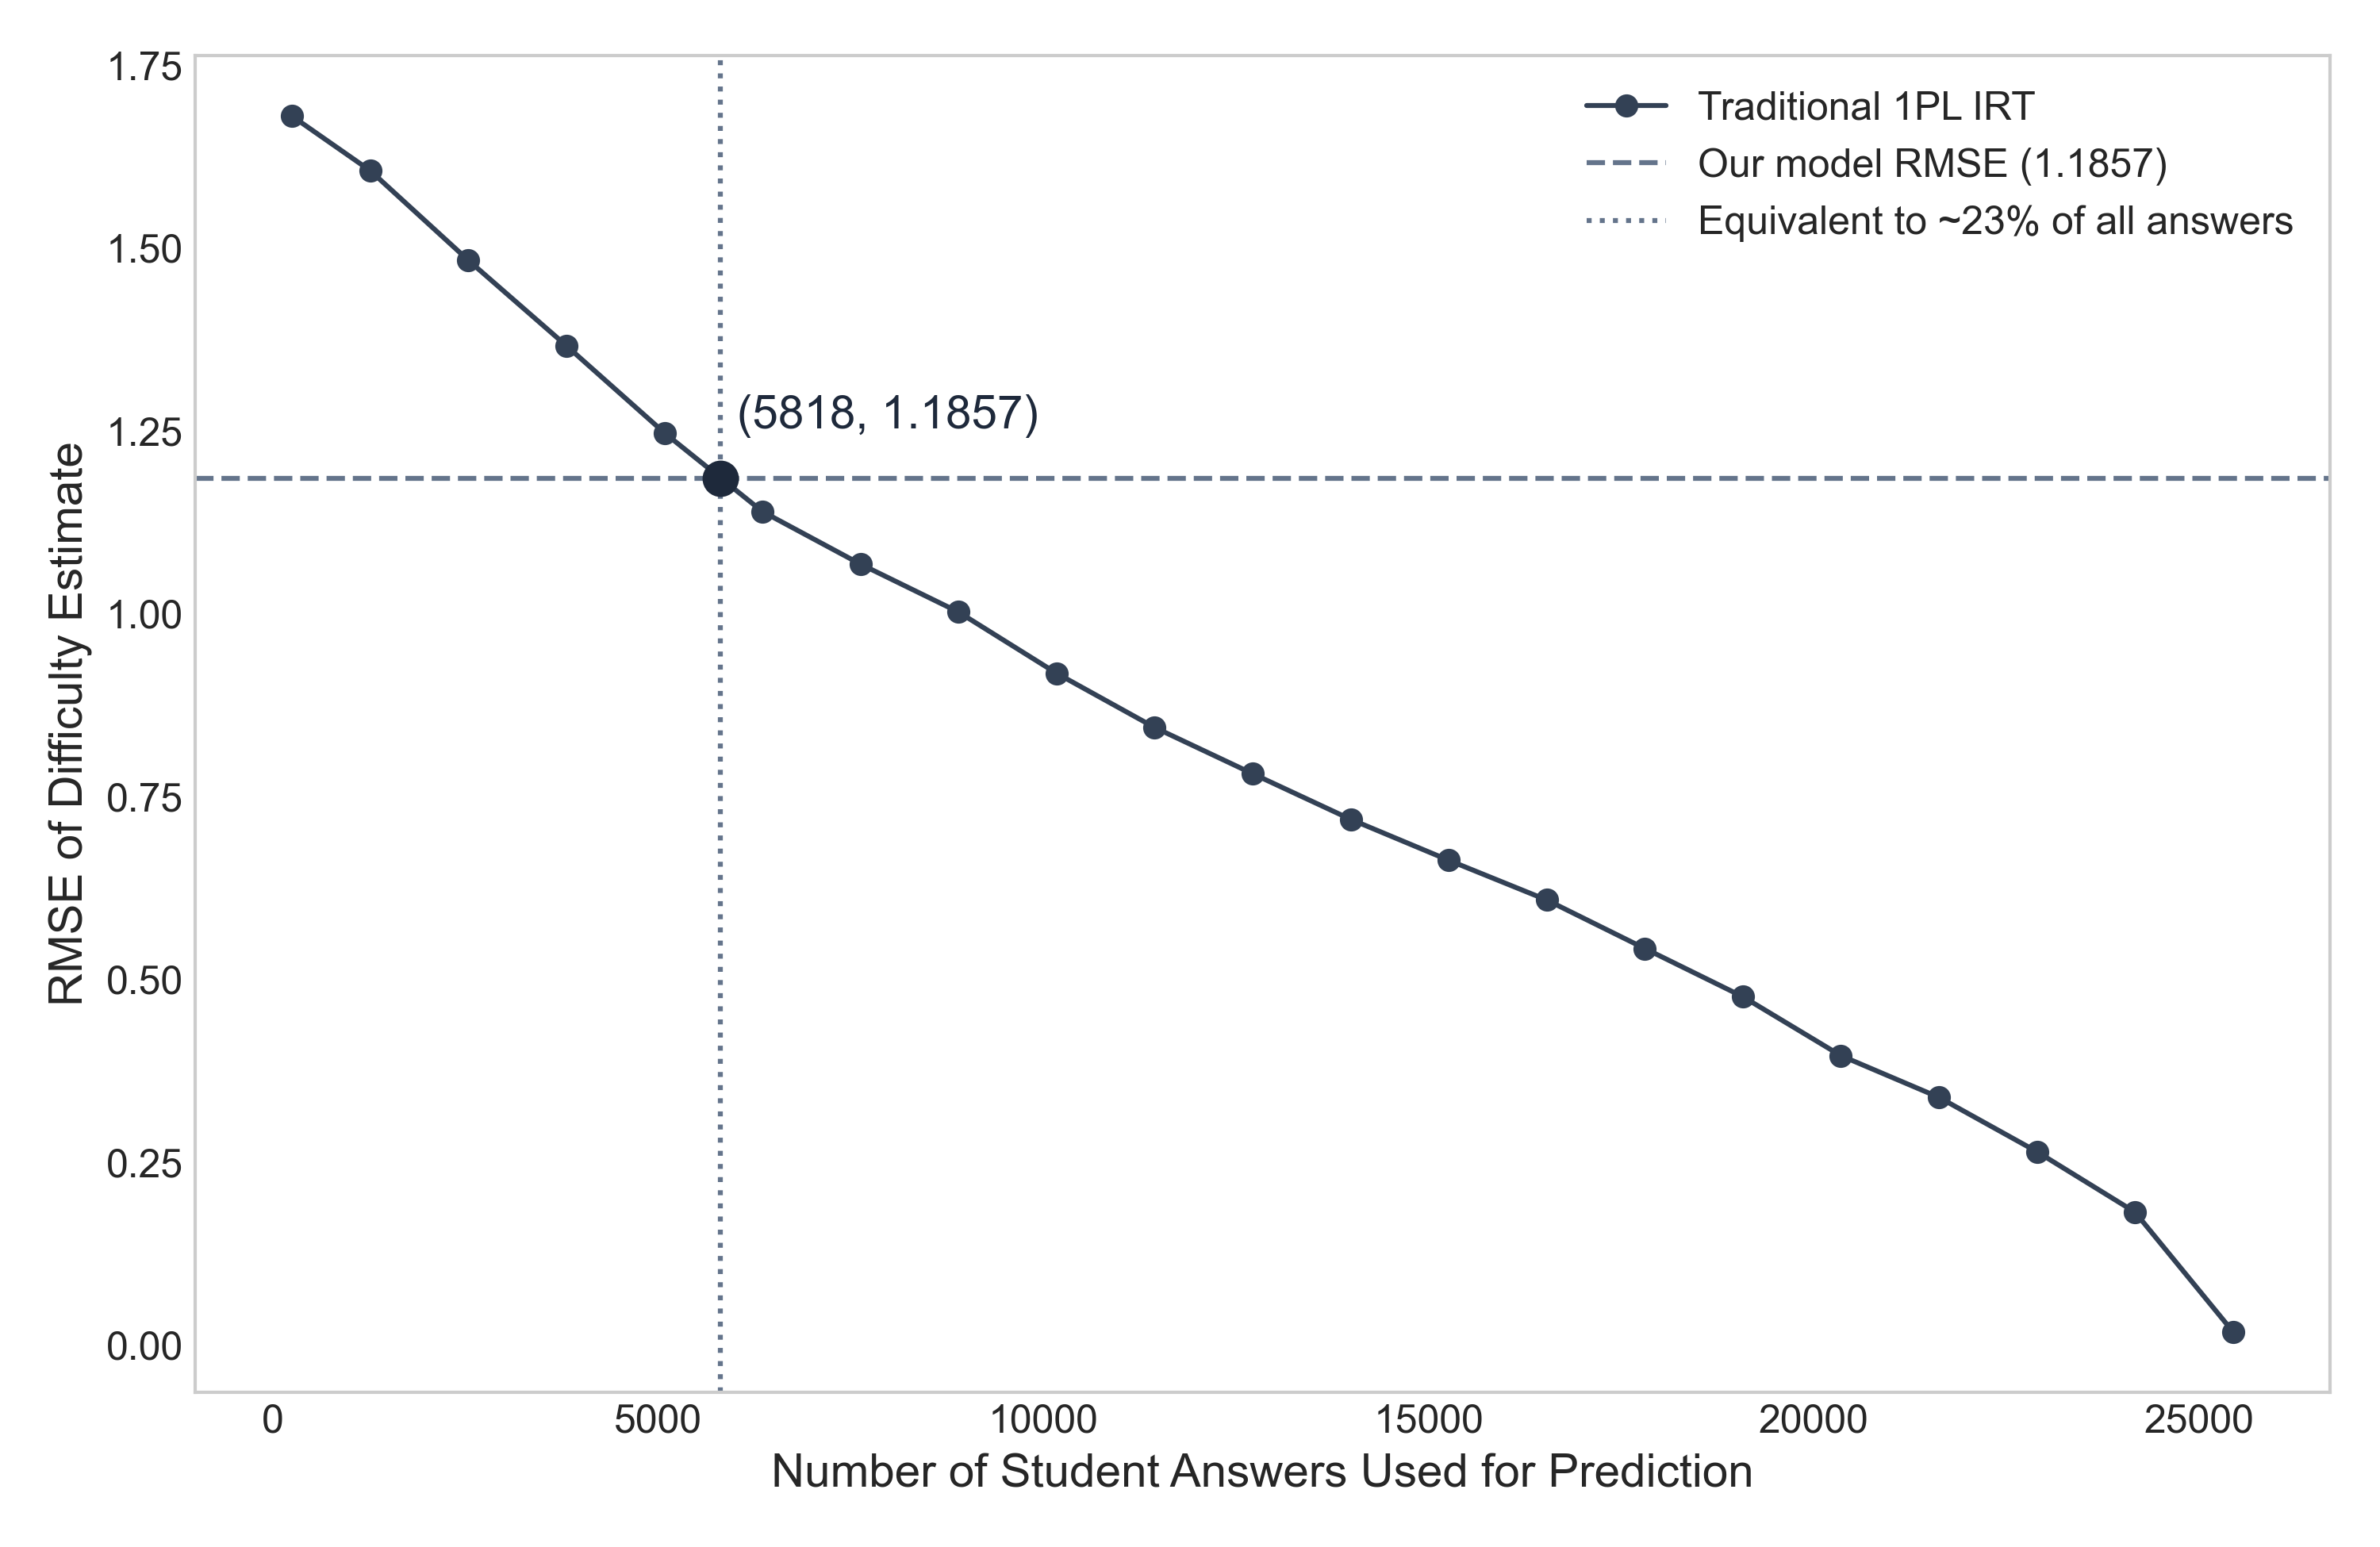
\includegraphics[width=1\columnwidth]{figures/rmse_efficiency_curve.png}
    \caption{RMSE-Based Efficiency of NN-Derived Difficulty Estimates compared to Traditional 1PL IRT using varying amounts of real student data.}
    \label{fig:rmse-efficiency}
\end{figure}

\begin{table}[H]
    \centering
    \begin{tabular}{ccc}
        \hline
        \textbf{\% Real Data Used} & \textbf{Approx. Answer Count} & \textbf{Simulated RMSE} \\
        \hline
        1.0\% & 254 & \textasciitilde1.6807 \\
        5.0\% & 1,272 & \textasciitilde1.6059 \\
        10.0\% & 2,544 & \textasciitilde1.4834 \\
        15.0\% & 3,816 & \textasciitilde1.3666 \\
        20.0\% & 5,088 & \textasciitilde1.2475 \\
        \textbf{Our Model's Performance} & \textbf{(NN-derived, ~5,818 equiv.)} & \textbf{1.1857} \\
        25.0\% & 6,360 & \textasciitilde1.1399 \\
        30.0\% & 7,632 & \textasciitilde1.0680 \\
        % ... (selected entries for brevity, can include more from strategy doc) ...
        50.0\% & 12,720 & \textasciitilde0.7815 \\
        100.0\% & 25,440 & \textasciitilde0.0185 \\
        \hline
    \end{tabular}
    \caption{RMSE of 1PL IRT difficulty estimates using varying amounts of real student data for 470 holdout questions, compared to NN-derived difficulty RMSE.}
    \label{tab:rmse-efficiency}
\end{table}

This evaluation indicates that our NN-derived 1PL difficulty estimates achieve an accuracy (RMSE of 1.1857) comparable to using approximately **5,818 real student answers** in a traditional 1PL IRT estimation for these same 470 holdout questions. This represents approximately **22.87\%** of the total available real responses for these items in the holdout set. This suggests a significant potential for data efficiency using our modeling approach.

\subsection{Feature Ablation Study}
To investigate the contribution of different feature types to the model's performance in predicting student correctness and subsequent IRT difficulty estimation, a feature ablation study was conducted. This study employed the same 1PL vs. 1PL comparison framework and neural network hyperparameters as our main reported model.

\subsubsection{Feature Buckets for Ablation Study}
Features were incrementally added to a baseline of text embeddings:
\begin{enumerate}
    \item \textbf{Model 1 (Embeddings Only)}: Utilized only the \texttt{nomic-ai/modernbert-embed-base} text embeddings of the formatted question text.
    \item \textbf{Model 2 (Embeddings + Question Features)}: Added linguistic and structural features derived from the question title and text (e.g., \texttt{question\_word\_count}, \texttt{has\_image}, \texttt{Has\_Abstract\_Symbols}). This corresponds to Bucket 1 in \texttt{modeling\_strategy.md}.
    \item \textbf{Model 3 (Embeddings + Question + Option Features)}: Added linguistic and structural features derived from the answer options (e.g., \texttt{jaccard\_similarity\_std}, \texttt{avg\_option\_length}, \texttt{Has\_NoneAll\_Option}). This corresponds to Bucket 1 + Bucket 2 in \texttt{modeling\_strategy.md}.
    \item \textbf{Model 4 (Embeddings + Question + Option + LLM Features)}: Added LLM-derived pedagogical features, both numerical (e.g., \texttt{avg\_steps}, \texttt{level}, \texttt{num\_misconceptions}, \texttt{Mathematical\_Notation\_Density}) and categorical (OHE: \texttt{Knowledge\_Dimension}, \texttt{Most\_Complex\_Number\_Type}, \texttt{Problem\_Archetype}). This corresponds to Bucket 1 + Bucket 2 + Bucket 3 in \texttt{modeling\_strategy.md} and represents the full feature set similar to our main reported model.
\end{enumerate}

\subsubsection{Ablation Results}
Table \ref{tab:ablation-results} summarizes the performance of these four models on the test set.

\begin{table}[H]
    \centering
    \resizebox{\columnwidth}{!}{
    \begin{tabular}{lccccc}
        \hline
        \textbf{Model Configuration} & \textbf{Test AUC} & \textbf{Test Acc.} & \textbf{Test F1} & \textbf{Pearson (1PL)} & \textbf{Spearman (1PL)} \\
        \hline
        Model 1: Embeddings Only & 0.7741 & 0.7518 & 0.8359 & 0.6822 & 0.7064 \\
        Model 2: Emb. + Question Feat. & 0.7743 & 0.7524 & 0.8351 & 0.6842 & 0.7065 \\
        Model 3: Emb. + Q \& Opt. Feat. & 0.7753 & 0.7513 & 0.8343 & 0.6758 & 0.7044 \\
        Model 4: Full Model (Emb. + Q \& Opt. + LLM) & 0.7818 & 0.7530 & 0.8351 & 0.7791 & 0.7606 \\
        \hline
    \end{tabular}
    }
    \caption{Feature ablation study results: correctness and 1PL vs. 1PL difficulty correlation metrics.}
    \label{tab:ablation-results}
\end{table}

\subsubsection{Ablation Study Conclusions}
This ablation study reveals the following insights:
\begin{itemize}
    \item \textbf{Baseline (Model 1: Embeddings Only):} Text embeddings alone achieve a Pearson correlation of \textasciitilde0.682 and Spearman of \textasciitilde0.706 for 1PL difficulty. Correctness AUC is \textasciitilde0.774.
    \item \textbf{Impact of Non-LLM Question and Option Features (Model 2 \& 3 vs. Model 1):} Adding traditional linguistic/structural question features (Model 2) maintained similar performance. Further adding option features (Model 3, which now includes embedding-derived option metrics) showed a slight dip in Pearson correlation (\textasciitilde0.676) but maintained Spearman correlation and AUC, suggesting these foundational features provide a stable base but don't dramatically lift performance over embeddings alone for difficulty correlation in this setup.
    \item \textbf{Impact of LLM-Derived Features (Model 4 vs. Model 3):} The most significant improvement came from adding the LLM-derived features. Model 4 (full model) showed a substantial increase in difficulty correlation (Pearson \textasciitilde0.779, Spearman \textasciitilde0.761) compared to Model 3. Correctness AUC also increased to \textasciitilde0.782. This highlights the strong contribution of the LLM-generated features for capturing nuances related to question difficulty.
\end{itemize}
These results underscore the significant contribution of the LLM-extracted features for capturing aspects of question difficulty that are not fully encompassed by text embeddings or basic structural/linguistic features alone. The full feature set in Model 4 demonstrates the strongest performance, aligning closely with our main reported model's capabilities.

\section{Discussion}

\subsection{Conclusions}

Our research demonstrates that Item Response Theory difficulty parameters can be accurately estimated without traditional student testing by combining linguistic features with pedagogical insights extracted using Large Language Models. The final model achieved a Pearson correlation of approximately 0.78 (Spearman correlation \textasciitilde0.76) between its predicted 1PL IRT difficulty parameters and benchmark 1PL parameters derived from actual student data, when evaluated on completely unseen questions. This approach addresses a significant challenge in educational assessment: the need for efficient methods to determine question difficulty that don't rely on resource-intensive pre-testing.

The strong performance of our neural network model in predicting student correctness (test set F1 score of 0.8350, AUC of 0.7789) confirms that our feature engineering approach effectively captures many factors influencing student performance. By integrating traditional linguistic and structural features, semantic embeddings of question text, and LLM-extracted pedagogical insights (such as solution step count, cognitive level, and misconception count), we created a rich representation of question characteristics.

Most importantly, the RMSE-based efficiency evaluation showed that our NN-derived 1PL difficulty estimates (RMSE of 1.1857 after scale alignment) are comparable in accuracy to using approximately 5,800 real student answers (representing about 22.87\% of the available data for the holdout questions) in a traditional 1PL IRT estimation. This highlights a substantial potential for data efficiency and cost reduction in assessment development.

Furthermore, the feature ablation study confirmed the significant contribution of LLM-derived pedagogical features. When added to a baseline of text embeddings and other non-LLM structural/lexical features, the LLM features provided a notable boost in the correlation between predicted and benchmark IRT difficulty parameters. This supports the claim that these advanced, AI-extracted features are valuable for capturing nuances of question difficulty.

These findings suggest that our simulation-based approach can reliably estimate question difficulty, potentially accelerating assessment development while maintaining psychometric quality, and opens new avenues for AI-assisted educational assessment design.

\subsection{Limitations}

Despite the promising results, several limitations of our study should be acknowledged:

\paragraph{Generalizability}: Our dataset originates from Chile, which may limit the generalizability of our findings to student populations elsewhere. Educational systems, curricula, and pedagogical approaches vary across countries and cultures, potentially affecting how question features relate to difficulty in different contexts.
    
\paragraph{LLM Stability}: Large Language Models are inherently probabilistic. Even though we attempted to ensure stability by making multiple LLM calls and aggregating results for features like `avg\_steps` and `num\_misconceptions`, each new call could potentially yield different outputs. This variability introduces some uncertainty into the LLM-extracted features, which could affect the consistency of our predictions.
    
\paragraph{Model Interpretability}: The neural network we employed is essentially a black box that performs well on the prediction task but offers limited insight into the relative importance of different features beyond what was shown in the ablation study. This makes it challenging to draw definitive conclusions about which specific question characteristics contribute most significantly to difficulty within the combined model.
    
\paragraph{Model Sensitivity}: Additionally, our results may vary depending on which LLM vendor we use (e.g., OpenAI, Anthropic, Google) and which inference parameters we select (e.g., temperature, top-p sampling). These choices can significantly impact the quality and consistency of the LLM-extracted features that feed into our model.

\subsection{Future Work}

In future iterations of this research, we plan to address these limitations through several targeted improvements:

\paragraph{Dataset Expansion}: We are currently in discussions to obtain the ASSISTments dataset to validate our approach on a different student population. This additional dataset would allow us to test the generalizability of our method across different educational contexts and student demographics.
    
\paragraph{Baseline Comparisons and Feature Analysis}: The feature ablation study provided initial insights. Further systematic removal or addition of specific LLM-derived features or other feature groups can help to more precisely quantify their individual and combined contributions to prediction accuracy and difficulty alignment. Comparing against simpler regression models using only subsets of features would also be beneficial.
    
\paragraph{Methodological Variations}: We will test variations of the model architecture, different LLM providers or versions for feature extraction, and alternative embedding models to evaluate the sensitivity of our results to these methodological choices. This exploration will help identify the most robust and effective configuration for difficulty prediction.
    
\paragraph{Refinement of LLM-Derived Pedagogical Features}: We plan to continue refining the LLM-based feature extraction process. This could involve exploring more sophisticated prompting techniques for features like `avg\_steps`, `level`, and `num\_misconceptions`, or investigating new types of pedagogical features that LLMs can extract to better capture question complexity.
    
\paragraph{Human Validation}: We will compare LLM annotations for features like cognitive level or misconception identification with human expert annotations for a subset of questions to assess the agreement between automated and human judgments. This validation will help establish the credibility of LLM-extracted features and identify areas where LLM performance could be improved.

By addressing these directions in future research, we aim to strengthen the validity, reliability, and generalizability of our approach to difficulty estimation, potentially establishing a new standard for efficient assessment development in educational contexts.

%----------------------------------------------------------------------------------------
% REFERENCES
%----------------------------------------------------------------------------------------
\printbibliography % Output the bibliography

%----------------------------------------------------------------------------------------
% APPENDICES
%----------------------------------------------------------------------------------------
\clearpage % Force a page break before the appendix

\appendix % This command switches to letter-based section numbering

% Redefine section and subsection formatting for appendix
\renewcommand{\thesection}{} % Remove section numbering completely
\renewcommand{\thesubsection}{\Alph{subsection}} % Use letters for subsections

% Change section title format to not show the number
\titleformat{\section}
  [block]
  {\Large\bfseries\centering}
  {}
  {0em}
  {}

\section{Appendix}

\subsection{Step by Step Example}
\label{sec:step-by-step-example}
The following is an example prompt used to generate step by step solution explanations for a mathematical problem:

\begin{questionbox}{Prompt}
    You are an expert in math pedagogy. Your task is to answer the following question deconstructing it to the most elemental steps. Don't skip any step. Don't assume anything about the reader, try to solve it in the most atomic and pedagogical way possible.

    \vspace{1em}
  
    Here is the question:
    \vspace{1em}

    Question: What is the decreasing order of the roots $4\sqrt{3}$, $3\sqrt{4}$, $2\sqrt{5}$, and $5\sqrt{2}$?  

    A) $2\sqrt5 > 4\sqrt3 > 5\sqrt2 > 3\sqrt4$

    B) $2\sqrt5 > 3\sqrt4 > 4\sqrt3 > 5\sqrt2$

    C) $5\sqrt2 > 3\sqrt4 > 4\sqrt3 > 2\sqrt5$

    D) $5\sqrt2 > 4\sqrt3 > 3\sqrt4 > 2\sqrt5$

    E) $2\sqrt5 > 4\sqrt3 > 5\sqrt2 > 3\sqrt4$

    Correct Answer: D

    \vspace{1em}

    First, think about your task step by step inside <thinking></thinking> tags. Your thinking process should try to go over all the posible ways to solve the question and try to find the most atomic way to solve it.

    \vspace{1em}

    Then, when you are ready to answer, after your </thinking> tag you should write your response using "Step" as the key and the step as the value. For example:

    \vspace{1em}

    <thinking>

      Thinking process... Think as long as you need to.

    </thinking>

    \vspace{1em}

    Step 1: ...

    Step 2: ...

    Step 3: ...

    ...

    \vspace{1em}

    Important instructions:

    - Don't skip any step.
    
    - Don't assume anything about the reader, try to solve it in the most atomic and pedagogical way possible.

    - Use as many steps as you need to.
\end{questionbox}

And here is the LLM's response:

\begin{studentbox}{Thinking Process}
    <thinking>

    Okay, let's break down this problem. We need to compare four numbers:  $4\sqrt{3}$, $3\sqrt{4}$, $2\sqrt{5}$, and $5\sqrt{2}$ and arrange them in decreasing order. The main challenge is that the numbers are in a mixed form (integer multiplied by a square root). To compare them easily, we need to get rid of the square roots or the integers outside the square root.

    \vspace{1em}

    The easiest way to compare these values is to bring the coefficients *inside* the square root.

    \vspace{1em}

    Let's consider how to bring a number inside a square root. For example, consider $a\sqrt{b}$. We can rewrite this as $\sqrt{a^2 * b}$.

    \vspace{1em}

    So, the first step is to convert all the numbers into the form of a single square root.

    \vspace{1em}

    Then, we simply compare the numbers *inside* the square roots, because if $a > b$, then $\sqrt{a} > \sqrt{b}$.

    \vspace{1em}

    Finally, we arrange the original numbers based on their corresponding squared values, in decreasing order.

    \vspace{1em}

    Let's start the solution.

    </thinking>

    \vspace{1em}
\end{studentbox}

\begin{llmbox}{Response}
    Step 1: Convert $4\sqrt{3}$ into the form $\sqrt{x}$.

    We have $4\sqrt{3} = \sqrt{4^2 * 3} = \sqrt{16 * 3} = \sqrt{48}$
    
    \vspace{1em}

    Step 2: Convert $3\sqrt{4}$ into the form $\sqrt{x}$.

    We have $3\sqrt{4} = \sqrt{3^2 * 4} = \sqrt{9 * 4} = \sqrt{36}$
    
    \vspace{1em}

    Step 3: Convert $2\sqrt{5}$ into the form $\sqrt{x}$.

    We have $2\sqrt{5} = \sqrt{2^2 * 5} = \sqrt{4 * 5} = \sqrt{20}$
    
    \vspace{1em}

    Step 4: Convert $5\sqrt{2}$ into the form $\sqrt{x}$.

    We have $5\sqrt{2} = \sqrt{5^2 * 2} = \sqrt{25 * 2} = \sqrt{50}$
    
    \vspace{1em}

    Step 5: Now we have $\sqrt{48}$, $\sqrt{36}$, $\sqrt{20}$, and $\sqrt{50}$. We can easily compare the values inside the square roots: 48, 36, 20, and 50.

    \vspace{1em}

    Step 6: Arrange the values inside the square roots in decreasing order:

    50 > 48 > 36 > 20

    \vspace{1em}

    Step 7: Replace the values inside the square roots with their original forms:

    $5\sqrt{2} > 4\sqrt{3} > 3\sqrt{4} > 2\sqrt{5}$

    \vspace{1em}

    Step 8: Compare this result with the given options.

    The correct option is D: $5\sqrt{2} > 4\sqrt{3} > 3\sqrt{4} > 2\sqrt{5}$.
\end{llmbox}

\subsection{Bloom's Cognitive Level Table}
Table \ref{tab:blooms-taxonomy} outlines Bloom's Taxonomy levels used to classify the cognitive demands of problems. Each level is an ordinal number in our feature encoding. The LLM was provided with this rubric and asked to determine the primary cognitive level for each question (feature: \texttt{level}).
\begin{table}[H]
    \centering
    \begin{tabular}{p{0.30\columnwidth}p{0.70\columnwidth}}
        \hline
        \textbf{Cognitive Level} & \textbf{Description} \\
        \hline
        Remember & Recall facts and basic concepts \\
        Understand & Explain ideas or concepts, interpret, summarize \\
        Apply & Use information in new situations, execute procedures \\
        Analyze & Draw connections among ideas, break down into parts \\
        Evaluate & Justify a stand or decision, verify, critique \\
        Create & Produce new or original work, design, construct \\
        \hline
    \end{tabular}
    \caption{Bloom's Taxonomy of cognitive levels applied to mathematical problem classification.}
    \label{tab:blooms-taxonomy}
\end{table}

\subsection{Example of Misconceptions List}
Following the example from the appendix \ref{sec:step-by-step-example}, here is one of the outputs of the LLM when asked about common misconceptions for the question in the example. The prompt for the \texttt{num\_misconceptions} feature asked the LLM to generate an exhaustive, atomic list of such misconceptions, and the count was averaged over runs.

\begin{enumerate}
    \item Students may confuse 'decreasing order' with 'increasing order', leading them to reverse the correct order of the numbers.
    \item Students might incorrectly apply the property $a\sqrt{b} = \sqrt{a^2 * b}$ by forgetting to square 'a' before multiplying by 'b', calculating it as $a\sqrt{b} = \sqrt{a * b}$.
    \item Students might make arithmetic errors when squaring the number outside the square root (e.g., calculating $4^2$ as 8 instead of 16).
    \item Students might make arithmetic errors in the multiplication step within the square root (e.g., calculating $16 * 3$ as 45 instead of 48).
    \item Students may believe that the magnitude of the number outside the square root is the primary determinant of the overall value, even if the value inside the square root is smaller (e.g., incorrectly assuming that $5\sqrt{2}$ is always greater than $2\sqrt{5}$ because 5 > 2).
    \item After correctly comparing the values under the square roots, students might forget to convert them back to their original forms when selecting the final answer, leading them to choose an option with the numbers under the square roots ordered.
    \item Students might make careless copying errors when transferring the correctly ordered expressions from their intermediate steps to the final answer choice.
    \item Students may lack a strong number sense regarding the approximate values of square roots, making it difficult to estimate and compare the values without performing the conversion to a common form.
    \item Students may struggle with the concept that irrational numbers can be ordered on a number line, treating them as inherently harder to compare than integers.
    \item Students might try to apply the square root individually to each term, incorrectly stating that $a\sqrt{b} = \sqrt{a} * \sqrt{b}$.
    \item Students might not understand what a root is and how it affects the order of the numbers.
\end{enumerate}

This was performed 3 times and then averaged the number of misconceptions for each question.

\subsection{LLM Feature Extraction Prompts}
\label{app:llm_prompts}
This section details the core prompts used with Google's Gemini models (primarily \texttt{gemini-2.0-flash}, with \texttt{gemini-2.5-flash} or \texttt{gemini-2.5-pro} for more complex tasks as noted) to extract various pedagogical features. Prompts generally included instructions for chain-of-thought reasoning (within \texttt{<thinking>...</thinking>} tags, not shown in core prompts below for brevity) and a strict JSON output format. Features were typically aggregated over multiple runs (usually 1 or 3) for stability. Question-specific content like \texttt{\$\{questionTitle\}} and \texttt{\$\{optionsJson\}} were dynamically inserted.

\subsubsection{Knowledge Dimension (Feature: \texttt{Knowledge\_Dimension})}
\label{app:prompt_knowledge_dimension}
\textbf{Model Used:} \texttt{gemini-2.0-flash} (1 run)
\begin{promptbox}
Analyze the following math question. What primary type of knowledge does it assess? Choose one:
- Factual: Recalling specific facts, definitions, formulas, or properties.
- Conceptual: Understanding relationships between concepts, interpreting information, explaining ideas, applying knowledge flexibly.
- Procedural: Executing a sequence of steps or applying a standard algorithm or method.

Question:
\$\{questionTitle\}

Options:
\$\{options.map(opt => `- \$\{opt\}`).join('\\n')\}

Think step-by-step about what the student needs to know or do. Is it mainly recall, understanding connections, or following steps? Then state the single best classification.
\end{promptbox}

\subsubsection{Information Gap (Feature: \texttt{Question\_Answer\_Info\_Gap})}
\label{app:prompt_info_gap}
\textbf{Model Used:} \texttt{gemini-2.5-flash} (3 runs, mean aggregated)
\begin{promptbox}
Analyze the following math question. How much information, knowledge, or reasoning *not explicitly stated* in the question text itself is required to arrive at the correct solution? Consider implicit assumptions, required prior knowledge (beyond basic arithmetic), or necessary intermediate reasoning steps.

Use this scale:
1 = None: The answer can be derived directly using only the information and numbers explicitly given.
2 = Low: Requires minimal prior knowledge (e.g., a common definition) or a single, obvious implicit step.
3 = Medium: Requires recall of specific formulas/theorems not given, multiple implicit reasoning steps, or interpretation of context.
4 = High: Requires significant external knowledge, complex synthesis of unstated information, or bridging substantial gaps in the problem statement.

Question:
\$\{questionTitle\}

Options:
\$\{options.map(opt => `- \$\{opt\}`).join('\\n')\}

Think step-by-step about the solution process. What external knowledge (formulas, theorems, concepts) is needed? What steps rely on implicit understanding? How large is the gap between the stated information and the required solution path?
\end{promptbox}

\subsubsection{Max Expression Nesting Depth (Feature: \texttt{Max\_Expression\_Nesting\_Depth})}
\label{app:prompt_nesting_depth}
\textbf{Model Used:} \texttt{gemini-2.5-flash} (3 runs, mode aggregated)
\begin{promptbox}
Analyze the mathematical expressions in the following text. Consider nested parentheses, functions (like sqrt), fractions, exponents, etc. What is the maximum nesting depth required to parse the most complex part of any expression?

For example:
- '2 + 3' has depth 0.
- 'sqrt(5)' has depth 1.
- '3 * (4 + 5)' has depth 1.
- 'sqrt(a + (b/c))' has depth 2 (division inside addition inside sqrt).
- '((a+b)\^2) / (c - d)' has depth 2.

Text:
\$\{questionTitle\}

Think step-by-step about the structure of each expression. Identify the most deeply nested part. Count the levels of nesting.
\end{promptbox}

\subsubsection{Most Complex Number Type (Feature: \texttt{Most\_Complex\_Number\_Type})}
\label{app:prompt_complex_number_type}
\textbf{Model Used:} \texttt{gemini-2.0-flash} (1 run)
\begin{promptbox}
Analyze the numbers involved in this math question, including those in the options.
Consider integers, decimals, fractions, roots/irrationals (like sqrt(2) or pi), and complex numbers (like 3+2i).
DO NOT consider abstract variables (like x) for this specific task.

Based on the following hierarchy of *numerical* complexity (lowest to highest):
1: Integer (e.g., 5, -2, 0)
2: Decimal (e.g., 3.14, -0.5)
3: Fraction (e.g., 1/2, 3/4)
4: Root/Irrational (e.g., sqrt(3), pi)
5: Complex Number (e.g., 2i, 1+i)

What is the HIGHEST level of numerical complexity present in the question or its options?

Question:
\$\{questionTitle\}

Options:
\$\{options.map(opt => `- \$\{opt\}`).join('\\n')\}

Think step-by-step. Identify the different types of numbers present. Determine the highest level reached according to the hierarchy. Ignore variables/abstract symbols.
\end{promptbox}

\subsubsection{Has Abstract Symbols (Feature: \texttt{Has\_Abstract\_Symbols})}
\label{app:prompt_has_abstract_symbols}
\textbf{Model Used:} \texttt{gemini-2.0-flash} (1 run, result to 1/0)
\begin{promptbox}
Does the following math question or its options contain abstract symbols representing variables or unknown quantities (e.g., x, y, a, ?, width, length)? Ignore standard mathematical operators, functions, units, and concrete numbers.

Question:
\$\{questionTitle\}

Options:
\$\{options.map(opt => `- \$\{opt\}`).join('\\n')\}

Think step-by-step. Look for letters or symbols used as variables.
\end{promptbox}

\subsubsection{Units Check (Feature: \texttt{Units\_Check})}
\label{app:prompt_units_check}
\textbf{Model Used:} \texttt{gemini-2.0-flash} (1 run, result to 1/0)
\begin{promptbox}
Does the following math question involve units of measurement (like meters, kg, dollars, seconds, etc.) in a way that might require attention to units or potential conversions to solve correctly?

Question:
\$\{questionTitle\}

Think step-by-step. Identify any units mentioned. Consider if conversions are needed.
\end{promptbox}

\subsubsection{Problem Archetype (Feature: \texttt{Problem\_Archetype})}
\label{app:prompt_problem_archetype}
\textbf{Model Used:} \texttt{gemini-2.5-pro} (1 run)
\begin{promptbox}
Classify the primary task or structure of the following math question. Choose the single best fit from this list:
- Word Problem - Calculation
- Equation Solving
- Geometric Reasoning/Proof
- Data Interpretation
- Conceptual Definition/Understanding
- Formula Application
- Pattern Recognition
- Other

Question:
\$\{questionTitle\}

Think step-by-step about what the question asks the student to *do*. What is the core task?
\end{promptbox}

\subsubsection{Real-World Context Flag (Feature: \texttt{RealWorld\_Context\_Flag})}
\label{app:prompt_realworld_flag}
\textbf{Model Used:} \texttt{gemini-2.0-flash} (1 run, result to 1/0)
\begin{promptbox}
Does the context of the following math question primarily involve a real-world scenario (e.g., shopping, measuring objects, physics situations, stories about people) OR is it presented in a purely abstract mathematical way (e.g., manipulating equations, asking about number properties, abstract geometry without context)?

Respond with either 'REALWORLD' or 'ABSTRACT'.

Question:
\$\{questionTitle\}

Think step-by-step about the setting and elements described in the question.
\end{promptbox}

\subsubsection{Ratio of Abstract to Concrete Symbols (Feature: \texttt{Ratio\_Abstract\_Concrete\_Symbols})}
\label{app:prompt_abstract_ratio}
\textbf{Model Used:} \texttt{gemini-2.0-flash} (1 run, calculates ratio from counts)
\begin{promptbox}
Analyze the mathematical content in the text below.
1. Count the number of concrete numerical values (e.g., 5, 3.14, -2, 1/2).
2. Count the number of abstract symbols representing variables or unknown quantities (e.g., x, y, a, ?, width).
Ignore standard mathematical operators (+, -, =), functions (sqrt), and units (m, kg).

Text:
\$\{questionTitle\}

Think step-by-step. List the concrete numbers found. List the abstract symbols found. Provide the counts.
\end{promptbox}

\subsubsection{Distractor Plausibility (Features: \texttt{LLM\_Distractor\_Plausibility\_Max}, \texttt{LLM\_Distractor\_Plausibility\_Mean})}
\label{app:prompt_distractor_plausibility}
\textbf{Model Used:} \texttt{gemini-2.5-flash} (3 runs, results aggregated for Mean and AvgMax)
\begin{promptbox}
Analyze the following math question and its options. The correct answer is '\$\{correctOption\}'.
For each INCORRECT option provided below, rate its plausibility as a potential answer that a student might mistakenly choose.
Use the following scale:
1 = Very Unlikely: The option is nonsensical or completely unrelated.
2 = Unlikely: The option results from a significant calculation error or conceptual misunderstanding.
3 = Possible: The option might result from a common calculation mistake or a minor misunderstanding.
4 = Plausible: The option is a common mistake or addresses a known misconception related to the question.
5 = Very Plausible: The option is highly tempting, potentially resulting from a subtle error or a very common misconception.

Question:
\$\{questionTitle\}

All Options:
\$\{allOptionsStr\}

Correct Answer: \$\{correctOption\}

Think step-by-step about why each incorrect option might be chosen or not. Consider common student errors for this type of problem. Then, provide the rating for each incorrect option.
\end{promptbox}


\end{document}

